
%% bare_jrnl.tex
%% V1.4a
%% 2014/09/17
%% by Michael Shell
%% see http://www.michaelshell.org/
%% for current contact information.
%%
%% This is a skeleton file demonstrating the use of IEEEtran.cls
%% (requires IEEEtran.cls version 1.8a or later) with an IEEE
%% journal paper.
%%
%% Support sites:
%% http://www.michaelshell.org/tex/ieeetran/
%% http://www.ctan.org/tex-archive/macros/latex/contrib/IEEEtran/
%% and
%% http://www.ieee.org/

%%*************************************************************************
%% Legal Notice:
%% This code is offered as-is without any warranty either expressed or
%% implied; without even the implied warranty of MERCHANTABILITY or
%% FITNESS FOR A PARTICULAR PURPOSE! 
%% User assumes all risk.
%% In no event shall IEEE or any contributor to this code be liable for
%% any damages or losses, including, but not limited to, incidental,
%% consequential, or any other damages, resulting from the use or misuse
%% of any information contained here.
%%
%% All comments are the opinions of their respective authors and are not
%% necessarily endorsed by the IEEE.
%%
%% This work is distributed under the LaTeX Project Public License (LPPL)
%% ( http://www.latex-project.org/ ) version 1.3, and may be freely used,
%% distributed and modified. A copy of the LPPL, version 1.3, is included
%% in the base LaTeX documentation of all distributions of LaTeX released
%% 2003/12/01 or later.
%% Retain all contribution notices and credits.
%% ** Modified files should be clearly indicated as such, including  **
%% ** renaming them and changing author support contact information. **
%%
%% File list of work: IEEEtran.cls, IEEEtran_HOWTO.pdf, bare_adv.tex,
%%                    bare_conf.tex, bare_jrnl.tex, bare_conf_compsoc.tex,
%%                    bare_jrnl_compsoc.tex, bare_jrnl_transmag.tex
%%*************************************************************************


% *** Authors should verify (and, if needed, correct) their LaTeX system  ***
% *** with the testflow diagnostic prior to trusting their LaTeX platform ***
% *** with production work. IEEE's font choices and paper sizes can       ***
% *** trigger bugs that do not appear when using other class files.       ***                          ***
% The testflow support page is at:
% http://www.michaelshell.org/tex/testflow/



%\documentclass[journal]{IEEEtran}
\documentclass[12pt, draftclsnofoot, onecolumn]{IEEEtran}
%
% If IEEEtran.cls has not been installed into the LaTeX system files,
% manually specify the path to it like:
% \documentclass[journal]{../sty/IEEEtran}

\usepackage[latin1]{inputenc}
\usepackage{amsfonts}
\usepackage{amssymb}
\usepackage{amsthm}
\usepackage{fullpage}
\usepackage{setspace}
\usepackage{graphicx}
%\usepackage[pdftex]{graphicx}
\usepackage{psfrag}
\usepackage{color}
\usepackage{epsfig}
%\usepackage{appendix}
\usepackage{caption}
\usepackage{cite}
\usepackage{ifpdf}
\usepackage[cmex10]{amsmath}
\usepackage{algorithmic}
\usepackage{array}
\usepackage{stfloats}
\usepackage{url}
\usepackage{fixltx2e}
\usepackage{setspace} 
\usepackage{diagbox}
\usepackage{subfigure}



% Some very useful LaTeX packages include:
% (uncomment the ones you want to load)


% *** MISC UTILITY PACKAGES ***
%
\usepackage{ifpdf}
% Heiko Oberdiek's ifpdf.sty is very useful if you need conditional
% compilation based on whether the output is pdf or dvi.
% usage:
% \ifpdf
%   % pdf code
% \else
%   % dvi code
% \fi
% The latest version of ifpdf.sty can be obtained from:
% http://www.ctan.org/tex-archive/macros/latex/contrib/oberdiek/
% Also, note that IEEEtran.cls V1.7 and later provides a builtin
% \ifCLASSINFOpdf conditional that works the same way.
% When switching from latex to pdflatex and vice-versa, the compiler may
% have to be run twice to clear warning/error messages.






% *** CITATION PACKAGES ***
%
\usepackage{cite}
% cite.sty was written by Donald Arseneau
% V1.6 and later of IEEEtran pre-defines the format of the cite.sty package
% \cite{} output to follow that of IEEE. Loading the cite package will
% result in citation numbers being automatically sorted and properly
% "compressed/ranged". e.g., [1], [9], [2], [7], [5], [6] without using
% cite.sty will become [1], [2], [5]--[7], [9] using cite.sty. cite.sty's
% \cite will automatically add leading space, if needed. Use cite.sty's
% noadjust option (cite.sty V3.8 and later) if you want to turn this off
% such as if a citation ever needs to be enclosed in parenthesis.
% cite.sty is already installed on most LaTeX systems. Be sure and use
% version 5.0 (2009-03-20) and later if using hyperref.sty.
% The latest version can be obtained at:
% http://www.ctan.org/tex-archive/macros/latex/contrib/cite/
% The documentation is contained in the cite.sty file itself.






% *** GRAPHICS RELATED PACKAGES ***
%
\ifCLASSINFOpdf
  % \usepackage[pdftex]{graphicx}
  % declare the path(s) where your graphic files are
  % \graphicspath{{../pdf/}{../jpeg/}}
  % and their extensions so you won't have to specify these with
  % every instance of \includegraphics
  % \DeclareGraphicsExtensions{.pdf,.jpeg,.png}
\else
  % or other class option (dvipsone, dvipdf, if not using dvips). graphicx
  % will default to the driver specified in the system graphics.cfg if no
  % driver is specified.
  % \usepackage[dvips]{graphicx}
  % declare the path(s) where your graphic files are
  % \graphicspath{{../eps/}}
  % and their extensions so you won't have to specify these with
  % every instance of \includegraphics
  % \DeclareGraphicsExtensions{.eps}
\fi
% graphicx was written by David Carlisle and Sebastian Rahtz. It is
% required if you want graphics, photos, etc. graphicx.sty is already
% installed on most LaTeX systems. The latest version and documentation
% can be obtained at: 
% http://www.ctan.org/tex-archive/macros/latex/required/graphics/
% Another good source of documentation is "Using Imported Graphics in
% LaTeX2e" by Keith Reckdahl which can be found at:
% http://www.ctan.org/tex-archive/info/epslatex/
%
% latex, and pdflatex in dvi mode, support graphics in encapsulated
% postscript (.eps) format. pdflatex in pdf mode supports graphics
% in .pdf, .jpeg, .png and .mps (metapost) formats. Users should ensure
% that all non-photo figures use a vector format (.eps, .pdf, .mps) and
% not a bitmapped formats (.jpeg, .png). IEEE frowns on bitmapped formats
% which can result in "jaggedy"/blurry rendering of lines and letters as
% well as large increases in file sizes.
%
% You can find documentation about the pdfTeX application at:
% http://www.tug.org/applications/pdftex





% *** MATH PACKAGES ***
%
\usepackage[cmex10]{amsmath}
% A popular package from the American Mathematical Society that provides
% many useful and powerful commands for dealing with mathematics. If using
% it, be sure to load this package with the cmex10 option to ensure that
% only type 1 fonts will utilized at all point sizes. Without this option,
% it is possible that some math symbols, particularly those within
% footnotes, will be rendered in bitmap form which will result in a
% document that can not be IEEE Xplore compliant!
%
% Also, note that the amsmath package sets \interdisplaylinepenalty to 10000
% thus preventing page breaks from occurring within multiline equations. Use:
%\interdisplaylinepenalty=2500
% after loading amsmath to restore such page breaks as IEEEtran.cls normally
% does. amsmath.sty is already installed on most LaTeX systems. The latest
% version and documentation can be obtained at:
% http://www.ctan.org/tex-archive/macros/latex/required/amslatex/math/





% *** SPECIALIZED LIST PACKAGES ***
%
\usepackage{algorithmic}
% algorithmic.sty was written by Peter Williams and Rogerio Brito.
% This package provides an algorithmic environment fo describing algorithms.
% You can use the algorithmic environment in-text or within a figure
% environment to provide for a floating algorithm. Do NOT use the algorithm
% floating environment provided by algorithm.sty (by the same authors) or
% algorithm2e.sty (by Christophe Fiorio) as IEEE does not use dedicated
% algorithm float types and packages that provide these will not provide
% correct IEEE style captions. The latest version and documentation of
% algorithmic.sty can be obtained at:
% http://www.ctan.org/tex-archive/macros/latex/contrib/algorithms/
% There is also a support site at:
% http://algorithms.berlios.de/index.html
% Also of interest may be the (relatively newer and more customizable)
% algorithmicx.sty package by Szasz Janos:
% http://www.ctan.org/tex-archive/macros/latex/contrib/algorithmicx/




% *** ALIGNMENT PACKAGES ***
%
\usepackage{array}
% Frank Mittelbach's and David Carlisle's array.sty patches and improves
% the standard LaTeX2e array and tabular environments to provide better
% appearance and additional user controls. As the default LaTeX2e table
% generation code is lacking to the point of almost being broken with
% respect to the quality of the end results, all users are strongly
% advised to use an enhanced (at the very least that provided by array.sty)
% set of table tools. array.sty is already installed on most systems. The
% latest version and documentation can be obtained at:
% http://www.ctan.org/tex-archive/macros/latex/required/tools/


% IEEEtran contains the IEEEeqnarray family of commands that can be used to
% generate multiline equations as well as matrices, tables, etc., of high
% quality.




% *** SUBFIGURE PACKAGES ***
%\ifCLASSOPTIONcompsoc
%  \usepackage[caption=false,font=normalsize,labelfont=sf,textfont=sf]{subfig}
%\else
%  \usepackage[caption=false,font=footnotesize]{subfig}
%\fi
% subfig.sty, written by Steven Douglas Cochran, is the modern replacement
% for subfigure.sty, the latter of which is no longer maintained and is
% incompatible with some LaTeX packages including fixltx2e. However,
% subfig.sty requires and automatically loads Axel Sommerfeldt's caption.sty
% which will override IEEEtran.cls' handling of captions and this will result
% in non-IEEE style figure/table captions. To prevent this problem, be sure
% and invoke subfig.sty's "caption=false" package option (available since
% subfig.sty version 1.3, 2005/06/28) as this is will preserve IEEEtran.cls
% handling of captions.
% Note that the Computer Society format requires a larger sans serif font
% than the serif footnote size font used in traditional IEEE formatting
% and thus the need to invoke different subfig.sty package options depending
% on whether compsoc mode has been enabled.
%
% The latest version and documentation of subfig.sty can be obtained at:
% http://www.ctan.org/tex-archive/macros/latex/contrib/subfig/




% *** FLOAT PACKAGES ***
%
\usepackage{fixltx2e}
% fixltx2e, the successor to the earlier fix2col.sty, was written by
% Frank Mittelbach and David Carlisle. This package corrects a few problems
% in the LaTeX2e kernel, the most notable of which is that in current
% LaTeX2e releases, the ordering of single and double column floats is not
% guaranteed to be preserved. Thus, an unpatched LaTeX2e can allow a
% single column figure to be placed prior to an earlier double column
% figure. The latest version and documentation can be found at:
% http://www.ctan.org/tex-archive/macros/latex/base/


%\usepackage{stfloats}
% stfloats.sty was written by Sigitas Tolusis. This package gives LaTeX2e
% the ability to do double column floats at the bottom of the page as well
% as the top. (e.g., "\begin{figure*}[!b]" is not normally possible in
% LaTeX2e). It also provides a command:
%\fnbelowfloat
% to enable the placement of footnotes below bottom floats (the standard
% LaTeX2e kernel puts them above bottom floats). This is an invasive package
% which rewrites many portions of the LaTeX2e float routines. It may not work
% with other packages that modify the LaTeX2e float routines. The latest
% version and documentation can be obtained at:
% http://www.ctan.org/tex-archive/macros/latex/contrib/sttools/
% Do not use the stfloats baselinefloat ability as IEEE does not allow
% \baselineskip to stretch. Authors submitting work to the IEEE should note
% that IEEE rarely uses double column equations and that authors should try
% to avoid such use. Do not be tempted to use the cuted.sty or midfloat.sty
% packages (also by Sigitas Tolusis) as IEEE does not format its papers in
% such ways.
% Do not attempt to use stfloats with fixltx2e as they are incompatible.
% Instead, use Morten Hogholm'a dblfloatfix which combines the features
% of both fixltx2e and stfloats:
%
% \usepackage{dblfloatfix}
% The latest version can be found at:
% http://www.ctan.org/tex-archive/macros/latex/contrib/dblfloatfix/




%\ifCLASSOPTIONcaptionsoff
%  \usepackage[nomarkers]{endfloat}
% \let\MYoriglatexcaption\caption
% \renewcommand{\caption}[2][\relax]{\MYoriglatexcaption[#2]{#2}}
%\fi
% endfloat.sty was written by James Darrell McCauley, Jeff Goldberg and 
% Axel Sommerfeldt. This package may be useful when used in conjunction with 
% IEEEtran.cls'  captionsoff option. Some IEEE journals/societies require that
% submissions have lists of figures/tables at the end of the paper and that
% figures/tables without any captions are placed on a page by themselves at
% the end of the document. If needed, the draftcls IEEEtran class option or
% \CLASSINPUTbaselinestretch interface can be used to increase the line
% spacing as well. Be sure and use the nomarkers option of endfloat to
% prevent endfloat from "marking" where the figures would have been placed
% in the text. The two hack lines of code above are a slight modification of
% that suggested by in the endfloat docs (section 8.4.1) to ensure that
% the full captions always appear in the list of figures/tables - even if
% the user used the short optional argument of \caption[]{}.
% IEEE papers do not typically make use of \caption[]'s optional argument,
% so this should not be an issue. A similar trick can be used to disable
% captions of packages such as subfig.sty that lack options to turn off
% the subcaptions:
% For subfig.sty:
% \let\MYorigsubfloat\subfloat
% \renewcommand{\subfloat}[2][\relax]{\MYorigsubfloat[]{#2}}
% However, the above trick will not work if both optional arguments of
% the \subfloat command are used. Furthermore, there needs to be a
% description of each subfigure *somewhere* and endfloat does not add
% subfigure captions to its list of figures. Thus, the best approach is to
% avoid the use of subfigure captions (many IEEE journals avoid them anyway)
% and instead reference/explain all the subfigures within the main caption.
% The latest version of endfloat.sty and its documentation can obtained at:
% http://www.ctan.org/tex-archive/macros/latex/contrib/endfloat/
%
% The IEEEtran \ifCLASSOPTIONcaptionsoff conditional can also be used
% later in the document, say, to conditionally put the References on a 
% page by themselves.




% *** PDF, URL AND HYPERLINK PACKAGES ***
%
\usepackage{url}
% url.sty was written by Donald Arseneau. It provides better support for
% handling and breaking URLs. url.sty is already installed on most LaTeX
% systems. The latest version and documentation can be obtained at:
% http://www.ctan.org/tex-archive/macros/latex/contrib/url/
% Basically, \url{my_url_here}.




% *** Do not adjust lengths that control margins, column widths, etc. ***
% *** Do not use packages that alter fonts (such as pslatex).         ***
% There should be no need to do such things with IEEEtran.cls V1.6 and later.
% (Unless specifically asked to do so by the journal or conference you plan
% to submit to, of course. )


% correct bad hyphenation here
\hyphenation{op-tical net-works semi-conduc-tor}


\begin{document}

%
% paper title
% Titles are generally capitalized except for words such as a, an, and, as,
% at, but, by, for, in, nor, of, on, or, the, to and up, which are usually
% not capitalized unless they are the first or last word of the title.
% Linebreaks \\ can be used within to get better formatting as desired.
% Do not put math or special symbols in the title.
\title{Report}

%
%
% author names and IEEE memberships
% note positions of commas and nonbreaking spaces ( ~ ) LaTeX will not break
% a structure at a ~ so this keeps an author's name from being broken across
% two lines.
% use \thanks{} to gain access to the first footnote area
% a separate \thanks must be used for each paragraph as LaTeX2e's \thanks
% was not built to handle multiple paragraphs
%
\author{Tianpei Chen\\
Department of Electrical and Computer Engineering\\
McGill University\\
\today}

%\author{Michael~Shell,~\IEEEmembership{Member,~IEEE,}
%        John~Doe,~\IEEEmembership{Fellow,~OSA,}
%        and~Jane~Doe,~\IEEEmembership{Life~Fellow,~IEEE}% <-this % stops a space
%\thanks{M. Shell is with the Department
%of Electrical and Computer Engineering, Georgia Institute of Technology, Atlanta,
%GA, 30332 USA e-mail: (see http://www.michaelshell.org/contact.html).}% <-this % stops a space
%\thanks{J. Doe and J. Doe are with Anonymous University.}% <-this % stops a space
%\thanks{Manuscript received April 19, 2005; revised September 17, 2014.}}

% note the % following the last \IEEEmembership and also \thanks - 
% these prevent an unwanted space from occurring between the last author name
% and the end of the author line. i.e., if you had this:
% 
% \author{....lastname \thanks{...} \thanks{...} }
%                     ^------------^------------^----Do not want these spaces!
%
% a space would be appended to the last name and could cause every name on that
% line to be shifted left slightly. This is one of those "LaTeX things". For
% instance, "\textbf{A} \textbf{B}" will typeset as "A B" not "AB". To get
% "AB" then you have to do: "\textbf{A}\textbf{B}"
% \thanks is no different in this regard, so shield the last } of each \thanks
% that ends a line with a % and do not let a space in before the next \thanks.
% Spaces after \IEEEmembership other than the last one are OK (and needed) as
% you are supposed to have spaces between the names. For what it is worth,
% this is a minor point as most people would not even notice if the said evil
% space somehow managed to creep in.



% The paper headers
%\markboth{Journal of \LaTeX\ Class Files,~Vol.~13, No.~9, September~2014}%
%{Shell \MakeLowercase{\textit{et al.}}: Bare Demo of IEEEtran.cls for Journals}
% The only time the second header will appear is for the odd numbered pages
% after the title page when using the twoside option.
% 
% *** Note that you probably will NOT want to include the author's ***
% *** name in the headers of peer review papers.                   ***
% You can use \ifCLASSOPTIONpeerreview for conditional compilation here if
% you desire.




% If you want to put a publisher's ID mark on the page you can do it like
% this:
%\IEEEpubid{0000--0000/00\$00.00~\copyright~2014 IEEE}
% Remember, if you use this you must call \IEEEpubidadjcol in the second
% column for its text to clear the IEEEpubid mark.



% use for special paper notices
%\IEEEspecialpapernotice{(Invited Paper)}




% make the title area
\maketitle

% As a general rule, do not put math, special symbols or citations
% in the abstract or keywords.
%\begin{abstract}
%The abstract goes here.
%\end{abstract}

% Note that keywords are not normally used for peerreview papers.
%\begin{IEEEkeywords}
%IEEEtran, journal, \LaTeX, paper, template.
%\end{IEEEkeywords}






% For peer review papers, you can put extra information on the cover
% page as needed:
% \ifCLASSOPTIONpeerreview
% \begin{center} \bfseries EDICS Category: 3-BBND \end{center}
% \fi
%
% For peerreview papers, this IEEEtran command inserts a page break and
% creates the second title. It will be ignored for other modes.
\IEEEpeerreviewmaketitle

%\begin{spacing}{2.5}

\section{Introduction}
% The very first letter is a 2 line initial drop letter followed
% by the rest of the first word in caps.
% 
% form to use if the first word consists of a single letter:
% \IEEEPARstart{A}{demo} file is ....
% 
% form to use if you need the single drop letter followed by
% normal text (unknown if ever used by IEEE):
% \IEEEPARstart{A}{}demo file is ....
% 
% Some journals put the first two words in caps:
% \IEEEPARstart{T}{his demo} file is ....
% 
% Here we have the typical use of a "T" for an initial drop letter
% and "HIS" in caps to complete the first word.
%\IEEEPARstart{T}{his} demo file is intended to serve as a ``starter file''
%for IEEE journal papers produced under \LaTeX\ using
%IEEEtran.cls version 1.8a and later.
% You must have at least 2 lines in the paragraph with the drop letter
% (should never be an issue)
%I wish you the best of success.

%\hfill mds
 
%\hfill September 17, 2014
Decoder is one of the key components of Multiple-Input Multiple-Output (MIMO) systems. Designing of high performance and low complexity detector has become a bottleneck of Large MIMO systems. 

Firmly grounded in framework of statistical learning theory, Support Vector Machine (SVM) is proposed in 1960s [ref vapnik], and of immense research and industry interest since 1990s. SVM is a powerful tool for supervised learning tasks such as classification, regression and prediction. Moreover, the kernel trick [ref learning with kernels SVM regularization] makes it possible to map data samples into higher dimensional feature space. Therefore SVM can deal with non-linear learning tasks. This makes SVM become a promising tool for complex real-world problems.
Based on the similar principle, $\epsilon$-Support Vector Regression (epsilon-SVR) [vapnik 1995, smola 2003], is developed.

Like SVM, epsilon-SVR first change primal objective function into dual optimization task, then solving the dual quadratic optimization problem. Typically this kind of problem can be solved by numerical quadratic optimization (QP) methods, however, they are computational costly. Decomposition methods, denotes a set of algorithms that divide the optimization variables (Lagrange multipliers) into two sets W and N, W is the work set and N contains the rest optimization variables.  In each iteration, only work set is updated for optimization while the other variables are fixed. Sequential Minimal Optimization (SMO) [ref A fast algorithm sequential minimal optimization] is an extreme case of decomposition methods which chooses dual Lagrange multiplier to optimize in each iteration. In each iteration, decomposition method can find an analytic optimal solution for work set, which makes the solver works much more faster than numerical QP algorithms. Decomposition methods can be employed to epsilon SVR by the similar manner.

  Bouloulis et employ Wirtinger’s calculus into Reproducing Kernel Hilbert Space (RKHS) so that expands real-SVM to pure complex SVM by exploiting complex kernel [ref complex support vector machine]. Based on this work, we construct a prototype of a complexity \$ performance controllable detector for large MIMO based on dual channel complex SVR. The detector can be divided into two parallel real SVR optimization problem which can be solved independently. Moreover, only real part of kernel matrix is needed in both channel. This means a large amount of computation can be reduced. 
  
  Steinwart et[ref SVM without offset] shows with a proper designed work set selection strategy, the approach that choosing double Lagrange multipliers can be much more faster than choosing single Lagrange multiplier without performance loss.
  
Based on the discrete time MIMO channel model, In our regression model, this CSVR-detector is constructed without offset, The offset in SVR imposes an additional linear quality constraint, which makes it necessary for decomposition methods such as Sequential Minimal Optimization to update more than one Lagrange multipliers in each iteration.

Therefore, for each real SVR without offset, in principle, only one variable is needed to be updated in each iteration, In our prototype, we propose a sequential single Lagrange multiplier search strategy that find two Lagrange multiplier sequentially, which can approximate the optimal dual Lagrange multiplier searching strategy. The former one only requires $O(n)$ searches in one iteration, while the optimal dual Lagrange multiplier strategy requires $O(n^{2})$ searches per iteration.  
%\subsection{Subsection Heading Here}
%Subsection text here.

% needed in second column of first page if using \IEEEpubid
%\IEEEpubidadjcol

%\subsubsection{Subsubsection Heading Here}
%Subsubsection text here.
\section{System Model}\label{system model}
  Consider a large MIMO uplink multiplexing system with $N_{t}$ users, each user has one transmit antenna. The number of receive antennas at Base Station (BS) is $N_{r}$, $N_{r}\geq N_{t}$. Typically large MIMO systems have hundreds of antennas at BS serving several tens of terminals, as shown in Fig {\ref{large MIMO uplink model}}.
  \begin{figure}
  \centering
  \def\svgwidth{\columnwidth}
  %\includegraphics[scale=•]{•}
  \input{largeMIMOuplink.pdf_tex}
  \caption{Large MIMO uplink system }
  \label{large MIMO uplink model}
  \end{figure}
    
  Uncoded binary information sequences, which are modulated to complex symbols, are transmitted by users over a flat fading channel. Using a discrete time model, $\mathbf{y}\in\mathbb{C}^{N_{r}\times 1}$ is the received symbol vector written as:
\begin{equation}
\mathbf{y}=\mathbf{H}\mathbf{s}+\mathbf{n},   \label{discrete time MIMO system}
\end{equation}
where $\mathbf{s}\in \mathbb{C}^{N_{t}}$ is the transmitted symbol vector, with components that are mutually independent and taken from a finite signal constellation alphabet $\mathbb{O}$ (e.g. 4-QAM, 16-QAM, 64-QAM) of size $M$. The possible transmitted symbol vectors $\mathbf{s}\in \mathbb{O}^{N_{t}}$, satisfy $\mathbb{E}[\mathbf{s}\mathbf{s}^{H}]=\mathbf{I}_{N_t}E_{s}$, where $E_{s}$ denotes the symbol average energy, and $\mathbb{E}[\cdot]$ denotes the expectation operation. Furthermore $\mathbf{H}\in \mathbb{C}^{N_{r}\times N_{t}}$ denotes the Rayleigh fading channel propagation matrix with independent identically distributed (i.i.d) circularly symmetric complex Gaussian zero mean components with unit variance. Finally, $\mathbf{n}\in \mathbb{C}^{N_{r}}$ is the additive white Gaussian noise (AWGN) vector with zero mean components and $\mathbb{E}[\mathbf{n}\mathbf{n}^{H}]=\mathbf{I}_{N_{r}}N_{0}$, where $N_{0}$ denotes the noise power spectrum density, and hence $\frac{E_{s}}{N_{0}}$ is the signal to noise ratio (SNR). 

  Assume the receiver has perfect channel state information (CSI), meaning that $ \mathbf{H}$ is known, as well as the SNR. The task of the MIMO decoder is to recover $\mathbf{s}$ based on $\mathbf{y}$ and $\mathbf{H}$.

\section{Brief Introduction to $\epsilon$-Support Vector Regression}\label{Introduce epsilon SVR}
Suppose we are given training data set $((\mathbf{x}_{1}, y_{1}),(\mathbf{x}_{2},y_{2}),\cdots,(\mathbf{x}_{l},y_{l}))$, $l$ denotes the number of training samples, $\mathbf{x}\in \mathbb{R}^{v}$ denotes input data vector, $v$ is the number of features in $\mathbf{x}$. $y$ denotes output. The regression model (either linear or non-linear regression) is given by 
\begin{equation}
y_{i}=\mathbf{w}^{T}\Phi(\mathbf{x}_{i})+b  \quad i\in 1\cdots l 
\label{equation1}
\end{equation} 
where $\mathbf{w}$ denotes regression coefficient vector, $\Phi(x)$ denotes the mapping of $\mathbf{x}$ to higher dimensional feature space. \ref{equation1}.

\begin{figure}
\centering
\def\svgwidth{\columnwidth}
\input{epsilon-SVR.pdf_tex}
\caption{}
\label{epsilon-SVR}
\end{figure}

Here we give the primal optimization problem directly
\begin{eqnarray}
\nonumber
\frac{1}{2}||\mathbf{w}||^{2}+\sum_{j=1}^{l}C_{i}(R(\xi_{i})+R(\hat{\xi}_{i}))\\
s.t. \left\{\begin{array}{ll}
y_{i}-\mathbf{w}^{T}\Phi(\mathbf{x}_{i})-b &\leq \epsilon+\xi_{i}\\
\mathbf{w}^{T}\Phi(\mathbf{x}_{i})+b-y_{i} &\leq \epsilon+\hat{\xi}_{i}\\
\epsilon, \xi,\hat{\xi} &\geq 0
\end{array}\right.
\label{primal optimization problem}
\end{eqnarray}
In \ref{primal optimization problem}, $\frac{1}{2}||\mathbf{w}||^{2}$ is the regularization term in order to ensure the flatness of regression model. $\epsilon$ denotes the precision, if the error between estimation and real output is less than $\epsilon$, As shown in Fig \ref{epsilon-SVR}, only those data points outside the shadow part, which is called $\epsilon$ tube, contribute to cost function. $\xi$ and $\hat{\xi}$ denote slack variables that cope with noise of input data set, $R(x)$ denotes cost function, the simplest cost function is $R(x)=x$, risk function is determined by the statistical distribution of noise \cite{A tutorial of Support Vector Regression}, for example if the noise subject to Gaussian distribution, the optimal cost function is $R(x)=\frac{1}{2}x^{2}$. $C\sum_{i=1}^{l}(\xi_{i}+\hat{\xi}_{i})$ denotes the penalty of noise, $C\in \mathbb{R}$ and $C\geq 0$ controls the trade off between regularization term and noise penalty term.

From the rationale of regularized risk function, let $f_{true}(\mathbf{x})$ denotes true regression function and $f_{estimate}(\mathbf{x})$, $c(\mathbf{x},y,f_{estimate}(\mathbf{x}))$ denotes the risk function, the regression model can be written as $y=f_{true}(\mathbf{x})+\xi$, $\xi$ denotes additive noise. Assume the data samples are i.i.d. Based on Maximum Likelihood (ML) principle we want to  
\begin{eqnarray}
\nonumber
maximize\quad \prod_{i=1}^{l}P(y_{i}|f_{estimation}(\mathbf{x}_{i}))&=maximize\quad \prod_{i=1}^{l}P(\xi_{i})\\
&=maximize\quad \prod_{i=1}^{l}P(y_{i}-f(\mathbf{x}_{i})),
\label{risk function1}
\end{eqnarray}
Take the logarithm of (\ref{risk function1}), we have
\begin{eqnarray}
maximize\quad \sum_{i=1}^{l}log(P(y_{i}-f_{estimation}(\mathbf{x}_{i}))),
\label{risk function2}
\end{eqnarray}
Therefore the $i$th risk function of $(\mathbf{x_{i}}, y_{i})$ can be written as 
\begin{eqnarray}
c(\mathbf{x}_{i}, y_{i}, f_{estimation}(\mathbf{x}_{i}))=-log(P(y_{i}-f_{estimation}(\mathbf{x}_{i}))).
\label{risk function3}
\end{eqnarray}
Thus the equivalent formula of (12) can be written as 
\begin{equation}
minimize\quad  \sum_{i=1}^{l}c(\mathbf{x}_{i}, y_{i}, f_{estimation}(\mathbf{x}_{i})),
\label{Total risk function}
\end{equation} 
In $\epsilon$-SVR, Vapnik's $\epsilon$-insensitive function, as shown in (\ref{Vepsilon}), is applied to (\ref{risk function3}).
\begin{eqnarray}
|x|_{\epsilon}=\left\{\begin{array}{ll}
0   &if\quad |x|<\epsilon\\
|x|-\epsilon  &otherwise\\
\end{array}\right.
\label{Vepsilon}
\end{eqnarray}
Thus the cost function in $\epsilon$-SVR can be written as 
\begin{equation}
\tilde{c}(\mathbf{x}, y, f_{estimation}(\mathbf{x}))=\frac{1}{l}\sum_{i=1}^{l}m_{i}(-log(P(|y_{i}-f_{estimation}(\mathbf{x}_{i})|_{\epsilon}))),
\label{cost function}
\end{equation}
where $m_{i}\in \mathbb{R}$, $m_{i}>0$ denotes the weight parameter, if $y_{i}>f_{estiamtion}(\mathbf{x})$, $m_{i}=m_{positive}$, else $m_{i}=m_{negative}$, Therefore the regularized risk function can written as 
\begin{equation}
minimize\quad \lambda||w||^{2}+\tilde{c}(\mathbf{x}, y, f_{estimation}(\mathbf{x})),
\label{total cost function}
\end{equation} 
where $\lambda$ denotes the weight of regularization term, divide (\ref{total cost function}) by $\frac{1}{2\lambda}$, we have the optimization problem  
\begin{equation}
minimize \quad \frac{1}{2}||w||^{2}+\sum_{i=1}^{l}C_{i}(-log(P(|y_{i}-f_{estimation}(\mathbf{x}_{i})|_{\epsilon}))),
\label{final cost function}
\end{equation}
where $C_{i}=\frac{m_{i}}{2\lambda l}$, based on (\ref{final cost function}), by introducing slack variables, we can easily derive the equivalent optimization problem as same as (\ref{primal optimization problem}):
\begin{eqnarray}
\nonumber
minimize \quad f(\mathbf{w})=\frac{1}{2}||\mathbf{w}||^{2}+\sum_{j=1}^{l}C_{i}(R(\xi_{i})+R(\hat{\xi}_{i}))\\
s.t. \left\{\begin{array}{ll}
y_{i}-\mathbf{w}^{T}\Phi(\mathbf{x}_{i})-b &\leq \epsilon+\xi_{i}\\
\mathbf{w}^{T}\Phi(\mathbf{x}_{i})+b-y_{i} &\leq \epsilon+\hat{\xi}_{i}\\
\epsilon, \xi,\hat{\xi} &\geq 0\\
\end{array}\right.
\label{primal objective function}
\end{eqnarray}
where $R(x)=-log(P(x))$, by this way, the discontinuity of $\epsilon$-insensitive function is conquered, we arrive to at a convex minimization problem \cite{smola and skpkof 1998a tutorial of SVR}. 

construct Lagrangian dual form of (\ref{primal optimization problem}) by introducing Lagrange multiplier,  dual optimization problem
\begin{eqnarray}
\nonumber
\min_{\alpha, \hat{\alpha}, \eta, \hat{\eta}, \mathbf{w}, \xi, \hat{\xi}}\Theta=
\frac{1}{2}||\mathbf{w}||^{2}+\sum_{j=1}^{l}C_{i}(R(\xi_{i})+R(\hat{\xi}_{i}))-\sum_{i=1}^{l}(\eta_{i}\xi_{i}+\hat{\eta}_{i}\hat{\xi}_{i})\\
\nonumber
-\sum_{i=1}^{l}\alpha_{i}(\epsilon+\xi_{i}-y_{i}+\mathbf{w}^{T}\Phi(\mathbf{x}_{i}))-\sum_{i=1}^{l}\hat{\alpha}_{i}(\epsilon+\hat{\xi}_{i}+y_{i}-\mathbf{w}^{T}\Phi(\mathbf{x}_{i}))\\
s.t. \left\{\begin{array}{cc}
\eta, \hat{\eta}, \alpha, \hat{\alpha}\geq 0\\
\xi, \hat{\xi}\geq  0\\
\end{array}\right. 
\label{lagrange duality1}
\end{eqnarray}
where $\eta$,$\hat{\eta}$, $\alpha$, $\hat{\alpha}$ are Lagrange multipliers.

According to Lagrangian Theorem \cite{Introduction to SVM}, the necessary condition to find the minimum of (\ref{primal objective function}) is the partial derivative of $\Theta$ with respect to $\mathbf{w}$, $\xi$, $\hat{\xi}$ and $b$ equal to $0$, 

\begin{equation}
\frac{\partial \theta}{\partial \mathbf{w}}=w-\sum_{i=1}^{l}(\alpha_{i}-\hat{\alpha}_{i})
\label{partial1}
\end{equation}

\begin{equation}
\frac{\partial \Theta}{\partial \xi}=C_{i}R^{'}(\xi_{i})-\eta_{i}-\alpha_{i}=0
\label{partial2}
\end{equation}

\begin{equation}
\frac{\partial \Theta}{\partial \hat{\xi}}=C_{i}R^{'}(\hat{\xi_{i}})-\hat{\eta}_{i}-\hat{\alpha}_{i}=0
\label{partial3}
\end{equation}

\begin{equation}
\frac{\partial \Theta}{\partial b}=\sum_{i=1}^{l}(\alpha_{i}-\hat{\alpha}_{i})=0
\label{partial4}
\end{equation} 
Then substitute (\ref{partial1})-(\ref{partial4}) to (\ref{lagrange duality2}) and for sake of brevity, we make $C_{i}$ uniform to all data samples, we have the dual form :
\begin{eqnarray}
\nonumber
\theta &=&\frac{1}{2}\sum_{i=1}^{l}\sum_{i=1}^{l}(\alpha_{i}-\hat{\alpha_{i}})(\alpha_{j}-\hat{\alpha_{j}})\Phi(\mathbf{x}_{j})^{T}\Phi(\mathbf{x}_{i})+C\sum_{i=1}^{l}[(R(\xi_{i})-\xi_{i}R^{'}(\xi_{i}))\\
\nonumber
&+&(R(\hat{\xi}_{i})-\hat{\xi}_{i}R^{'}(\hat{\xi}_{i}))]
+\sum_{i=1}^{l}[(\alpha_{i}-\hat{\alpha_{i}})y_{i}-(\alpha_{i}+\hat{\alpha_{i}})\epsilon]\\
\nonumber
&-&\sum_{i=1}^{l}\sum_{i=1}^{l}(\alpha_{i}-\hat{\alpha_{i}})(\alpha_{j}-\hat{\alpha_{j}})\Phi(\mathbf{x}_{j})^{T}\Phi(\mathbf{x}_{i}),\\
&s.t.&\left\{\begin{array}{l}
\sum_{i=1}^{l}(\alpha_{i}-\hat{\alpha_{i}})=0\\
0<\alpha<C\tilde{R}^{'}(\alpha)\\
0<\hat{\alpha}<C\tilde{R}^{'}(\hat{\alpha})\\
\end{array}\right.
\label{dual objective function1}
\end{eqnarray}
Thus $\theta(\alpha,\hat{\alpha})\leq \Theta(\mathbf{w},\alpha, \hat{\alpha}, \eta, \hat{\eta})$, according to general Lagrange function\cite{introduction to SVM}, Lagrange duality with feasible solution always less or equal to original objective function, because inequality constraints is introduced. Therefore we have $\theta\leq \Theta \leq f(\mathbf{w})$, based on the lemma 5.16 of Lagrange theorem\cite{introduction of SVM}, the upper bound of $\theta$ is given by the minimal of $f(\mathbf{w})$, equality holds only when the optimal of $f(\mathbf{w})$ is obtained (property 5.19).
Therefore the Lagrangian duality form can be written as 
\begin{eqnarray}
\nonumber
maximize\quad \Theta &=&-\frac{1}{2}\sum_{i=1}^{l}\sum_{i=1}^{l}(\alpha_{i}-\hat{\alpha_{i}})(\alpha_{j}-\hat{\alpha_{j}})\Phi(\mathbf{x}_{j})^{T}\Phi(\mathbf{x}_{i})+\sum_{i=i}^{l}[(\alpha_{i}-\hat{\alpha_{i}})y_{i}-(\alpha_{i}+\hat{\alpha_{i}})\epsilon]\\
\nonumber
&+&C\sum_{i=1}^{l}[\tilde{R}(\xi_{i})+\tilde{R}(\hat{\xi_{i}})]\\
&=&-\frac{1}{2}(\mathbf{a}-\mathbf{\hat{a}})^{T}\mathbf{K}(\mathbf{a}-\mathbf{\hat{a}})+(\mathbf{y}-\epsilon)^{T}\mathbf{a}+(-\mathbf{y}-\epsilon)^{T}\mathbf{\hat{a}}+\mathbf{e}^{T}C(\tilde{R}(\xi)+\tilde{R}(\hat{\xi})),
\label{dual optimization function2}
\end{eqnarray}
where $\mathbf{a}=[\alpha_{1},\alpha_{2}, \ldots, \alpha_{l}]^{T} $, $\mathbf{\hat{a}}=[\hat{\alpha}_{1},\hat{\alpha}_{2}, \ldots, \hat{\alpha}_{l}]^{T} $, $\mathbf{y}=[y_{1}, y_{2}, \ldots y_{l}]^{T}$, $ \mathbf{e}=[1,1,\ldots,1]^{T}\in \mathbb{R}^{l}$, $\mathbf{e}_{i}$ denotes the vector that only $i$th component is 1 while the rest are all 0,  $\tilde{R}(\xi)=R(\xi)-\xi R^{'}(\xi)\in \mathbb{R}^{l}$, $\mathbf{K}_{ij}=\Phi(\mathbf{x}_{j})^{T}\Phi(\mathbf{x}_{i})$ denotes data kernel matrix. We define the following $2l$ vectors 
$\mathbf{a}^{(*)}$= [$\mathbf{a} \atop \mathbf{\hat{a}}$], $\mathbf{v}\in \mathbb{R}^{2l}$, 
\begin{eqnarray}
\mathbf{v}_{i}=\left\{\begin{array}{ll}
1\quad i=1,\ldots, l\\
-1\quad i=l+1,\ldots, 2l\\ 
\end{array}\right.
\end{eqnarray}
(\ref{dual optimization function2}) can be reformulate as 
\newcommand{\mysmallarraydecl}{\renewcommand{%
\IEEEeqnarraymathstyle}{\scriptscriptstyle}%
\renewcommand{\IEEEeqnarraytextstyle}{\scriptsize}%
\renewcommand{\baselinestretch}{1.1}%
\settowidth{\normalbaselineskip}{\scriptsize
\hspace{\baselinestretch\baselineskip}}%
\setlength{\baselineskip}{\normalbaselineskip}%
\setlength{\jot}{0.25\normalbaselineskip}%
\setlength{\arraycolsep}{2pt}}
\begin{equation}
maximize\quad \Theta=-\frac{1}{2}(\mathbf{a}^{*})^{T}\left[\begin{IEEEeqnarraybox*}[\mysmallarraydecl][c]{,c/c,}
\mathbf{K}& -\mathbf{K}\\
-\mathbf{K}& \mathbf{K}
\end{IEEEeqnarraybox*}\right]
\mathbf{a}^{(*)}+[(\mathbf{y}-\epsilon)^{T}, (-\mathbf{y}-\epsilon)^{T}]\mathbf{a}^{(*)}+\mathbf{e}^{T}C(\tilde{R}(\xi)+\tilde{R}(\hat{\xi})),
\label{vectorize dual optimization function}
\end{equation}


 
\section{Dual Channel Real Kernel Complex Support Vector Regression for Large MIMO system}\label{dual channel CSVR}
 Based on discrete time model of large MIMO uplink system in (\ref{discrete time MIMO system}), in our  regression model, the training data sample at detector is $(\mathbf{h}_{1}, y_{1})(\mathbf{h}_{2}, y_{2}), \ldots, (\mathbf{h}_{N_{r}}, y_{N_{r}})$, where $\mathbf{h}_{i}$ denotes $i$th row of channel propagation matrix $\mathbf{H}$, this yields a regression task without offset $b$:  
 \begin{eqnarray}
 y_{i}=f_{true}(\mathbf{h}_{i})+n,\\
 \label{regression part1a}
 f_{true}(\mathbf{h}_{i})=\mathbf{h}_{i}\mathbf{s},\\
 \label{regression part1b}
 \end{eqnarray}
 where $f_{true}()$ denotes the true regression function, $n$ denotes additive noise.
In this regression problem, receive symbol $y$ is the output data, $\mathbf{h}$ is input data sample, transmitted symbol vector $s$ is regression coefficients. Because the large MIMO system we consider here is complex, we employ complex support vector regression (CSVR) without offset term $b$. As shown in section \ref{Introduce epsilon SVR}, in order to derive Lagrange duality optimization formula, partial derivatives of objective function with respect to $\mathbf{w}$ and $\xi$ are needed to be calculated, in CSVR, that means take partial derivatives to real cost functions which are defined in complex domain. The recent mathematical results of Wirtinger's calculus in Reproducing Kernel Hilbert Space (RKHS)[\cite{wirtinger's calculus}][\cite {reproducing Kernel Hilbert Space}] is employed to solve this problem. First we generalize our regression model by complex RKHS, 
Let $<,>_{H}$ denotes inner product operation in real RKHS. $<,>_{\mathbb{H}}$ denotes inner products operation in complex RKHS. Assume $\mathbf{x}$, $\mathbf{y}$, $\mathbf{z}$, $j$, $k$ $\in \mathbb{C}$, complex Hilbert space has the following properties 
\newtheorem{Lemma}{Lemma}
\newtheorem{Property}{Property}
\begin{Property}
 $<\mathbf{x},\mathbf{y}>_{\mathbb{H}}=<\overline{\mathbf{y},\mathbf{x}}>_{\mathbb{H}}$
\label{CHSProperty1}
\end{Property}

\begin{Property}
$<j\mathbf{x}+k\mathbf{y},\mathbf{z}>_{\mathbb{H}}=j<\mathbf{x},\mathbf{z}>_{\mathbb{H}}+k<\mathbf{y},\mathbf{z}>_{\mathbb{H}}$
\label{CHSProperty2}
\end{Property}

\begin{Property}
$<\mathbf{z}, j\mathbf{x}+k\mathbf{y}>=\bar{j}<\mathbf{z},\mathbf{x}>_{\mathbb{H}}+\bar{k}<\mathbf{z}, \mathbf{y}>_{\mathbb{H}}$
\label{CHSProperty3}
\end{Property}

\begin{Lemma}
$\mathbf{h}_{i}\mathbf{s}\in <\mathbf{h}_{i},\mathbf{s}^{*}>_{\mathbb{H}}$
\end{Lemma}    

\begin{proof}
Assume $\mathbf{a}$, $\mathbf{b}$ $\in \mathbb{R}^{v}$, it can be easily proved  
\begin{equation}
\mathbf{a}^{T}\mathbf{b} \in <\mathbf{a}, \mathbf{b}>_{H},
\label{CHSequation1}
\end{equation}
 From Property \ref{CHSProperty1} and Property \ref{CHSProperty3}, it is obvious 
\begin{equation}
<\mathbf{g},\mathbf{h}>_{\mathbb{H}}=<\mathbf{g}^{r},\mathbf{h}^{r}>_{H}+<\mathbf{g}^{i},\mathbf{h}^{i}>_{H}+i(<\mathbf{g}^{i},\mathbf{h}^{r}>_{H}-<\mathbf{g}^{r},\mathbf{h}^{i}>_{H})
\label{CHSProperty4}
\end{equation}
where $\mathbf{g}$,$\mathbf{h}$ $\in \mathbb{C}^{v}$, and $\mathbf{g}=\mathbf{g}^{r}+i\mathbf{g}^{i}$, $\mathbf{h}=\mathbf{h}^{r}+i\mathbf{h}^{i}$. Therefore, 
\begin{eqnarray}
\nonumber
<\mathbf{h}, \mathbf{s}^{*}>_{\mathbb{H}}&=&<\mathbf{h}^{r},  (\mathbf{s}^{*})^{r}>_{H}+<\mathbf{h}^{i},  (\mathbf{s}^{*})^{i}>_{H}+i(<\mathbf{h}^{i},  (\mathbf{s}^{*})^{r}>_{H}-<\mathbf{h}^{r},  (\mathbf{s}^{*})^{i}>_{H})\\
&=&<\mathbf{h}^{r}, \mathbf{s}^{r}>_{H}-<\mathbf{h}^{i}, \mathbf{s}^{i}>_{H}+i(<\mathbf{h}^{i}, \mathbf{s}^{r}>_{H}+<\mathbf{h}^{r}, \mathbf{s}^{i}>_{H}),
\label{CHSequation2}
\end{eqnarray}

\begin{equation}
\mathbf{h}\mathbf{s}=\mathbf{h}^{r}\mathbf{s}^{r}-\mathbf{h}^{i}\mathbf{s}^{i}+i(\mathbf{h}^{i}\mathbf{s}^{r}+\mathbf{h}^{r}\mathbf{s}^{i}),
\label{CHSequation3}
\end{equation}
Because of (\ref{CHSequation1}), (\ref{CHSequation2}) and (\ref{CHSequation3}), $\mathbf{h}_{i}\mathbf{s}\in <\mathbf{h}_{i},\mathbf{s}^{*}>_{\mathbb{H}}$
\end{proof}
represent $\mathbf{s}^{*}$ by $\mathbf{w}$, The general regularized risk function of large MIMO detection in complex RKHS can be formulated:
\begin{eqnarray}
\nonumber
minimize \quad \frac{1}{2}||w||_{\mathbb{H}}^{2}+C\sum_{k=1}^{N_{r}}[(R(\xi^{r}_{k})+R(\hat{\xi}^{r}_{k})+R(\xi^{i}_{k})+R(\hat{\xi}^{i}_{k}))]\\
s.t. \left\{\begin{array}{ll}
Re(y_{k}-<\mathbf{h}_{k},\mathbf{w}>_{\mathbb{H}})\leq \epsilon+\xi^{r}_{k}\\
Re(<\mathbf{h}_{k},\mathbf{w}>_{\mathbb{H}}-y_{k})\leq \epsilon+\hat{\xi}^{r}_{k}\\
Im(y_{k}-<\mathbf{h}_{k},\mathbf{w}>_{\mathbb{H}})\leq \epsilon+\xi^{i}_{k}\\
Im(<\mathbf{h}_{k},\mathbf{w}>_{\mathbb{H}}-y_{k})\leq \epsilon+\hat{\xi}^{i}_{k}\\
\xi^{r}, \hat{\xi}^{r},\xi^{i},\hat{\xi}^{i}\geq 0\\
\end{array}\right.
\label{complex objective function1}
\end{eqnarray}
where $Re()$ and $Im()$ denote real part and imaginary part of a complex variable, restrictions are set to real and imaginary part of regression function separately. Let $\mathbf{K}=\mathbf{H}\mathbf{H}^{H}$ denotes the kernel function, $\mathbf{K}=\mathbf{K}^{r}+i\mathbf{K}^{i}$, $\mathbf{K}^{r}$ and $\mathbf{K}^{i}$ denote matrix of corresponding real part and imaginary part. Similar to the Lagrange duality rational in (\ref{lagrange duality2}), Lagrange duality is formulated for (\ref{complex objective function1}) 
\begin{IEEEeqnarray}[\relax]{l}
\nonumber
\max_{(\alpha, \hat{\alpha}, \beta, \hat{\beta}, \eta, \hat{\eta}, \tau, \hat{\tau})} \min_{(\mathbf{w}, \xi^{r}, \hat{\xi}^{r}, \hat{\xi}^{i}, \hat{\xi}^{i})} \theta =
\frac{1}{2}||w||_{\mathbb{H}}^{2}+C\sum_{k=1}^{N_{r}}[(R(\xi^{r}_{k})+R(\hat{\xi}^{r}_{k})+R(\xi^{i}_{k})+R(\hat{\xi}^{i}_{k}))]- \sum_{k=1}^{N_{r}}(\eta_{i}\xi^{r}_{k}+\hat{\eta}_{k}\hat{\xi}^{r}_{k}\\
\nonumber
+\tau_{k}\xi^{i}_{k}+\hat{\tau}_{k}\hat{\xi}^{i}_{k})-\sum_{k=1}^{N_{r}}\alpha_{k}(\epsilon+\xi^{r}_{k}-Re(y_{k})+Re(<\mathbf{h}_{k},\mathbf{w}>_{\mathbb{H}}))
-\sum_{k=1}^{N_{r}}\hat{\alpha}_{k}(\epsilon+\hat{\xi}^{r}_{k}+Re(y_{k})-Re(<\mathbf{h}_{k},\mathbf{w}>_{\mathbb{H}}))\\
\nonumber
-\sum_{k=1}^{N_{r}}\beta_{k}(\epsilon+\xi^{i}_{k}-Im(y_{k})+Im(<\mathbf{h}_{k},\mathbf{w}>_{\mathbb{H}}))-\sum_{k=1}^{N_{r}}\hat{\beta}_{k}(\epsilon+\hat{\xi}^{i}_{k}+Im(y_{k})-Im(<\mathbf{h}_{k},\mathbf{w}>_{\mathbb{H}}))\\
s.t. \left\{\begin{array}{ll}
\eta, \hat{\eta}, \tau, \hat{\tau} \alpha, \hat{\alpha}, \beta, \hat{\beta}\geq 0\\
\xi^{r}, \hat{\xi}^{r}, \xi^{i}, \hat{\xi}^{i} \geq  0
\end{array}\right. 
\label{complex lagrange duality1}
\end{IEEEeqnarray}
with Wirtinger's calculus applied to RKHS described in \cite{wirtinger's calculus to RKHS}, The partial derivatives of $\Theta$ respect to $\mathbf{w}$, which is define at complex domain, as well as the real variables $\xi^{r}$, $\hat{\xi}^{r}$, $\xi^{i}$ and $\hat{\xi}^{i}$ can be deduced 
\begin{IEEEeqnarray}[\relax]{l}
\left\{\begin{array}{ll}
\frac{\partial \Theta}{\partial \mathbf{w}^{*}}=\frac{1}{2}\mathbf{w}-\frac{1}{2}\sum_{k=1}^{N_{r}}\alpha_{k}\mathbf{h}_{k}+\frac{1}{2}\sum_{k=1}^{N_{r}}\hat{\alpha}_{k}\mathbf{h}_{k}+\frac{i}{2}(\sum_{k=1}^{N_{r}}\beta_{k}\mathbf{h}_{k}-\sum_{k=1}^{N_{r}}\hat{\beta}_{k}\mathbf{h}_{k})=0\\
\Rightarrow \mathbf{w}=\sum_{k=1}^{N_{r}}(\alpha_{k}-\hat{\alpha}_{k})\mathbf{h}_{k}-i\sum_{k=1}^{N_{r}}(\beta_{k}-\hat{\beta}_{k})\mathbf{h}_{k}\\
\frac{\partial \Theta}{\partial \xi^{r}_{k}}=CR^{'}(\xi^{r}_{k})-\eta_{k}-\alpha_{k}=0\Rightarrow \eta_{k}=CR^{'}(\xi^{r}_{k})-\alpha_{k}\\
\frac{\partial \Theta}{\partial \hat{\xi}^{r}_{k}}=CR^{'}(\hat{\xi}^{r}_{k})-\hat{\eta}_{k}-\hat{\alpha}_{k}=0\Rightarrow \hat{\eta}_{k}=CR^{'}(\hat{\xi}^{r}_{k})-\hat{\alpha}_{k}\\
\frac{\partial \Theta}{\partial \xi^{i}_{k}}=CR^{'}(\xi^{i}_{k})-\tau_{k}-\beta_{k}=0\Rightarrow \tau_{k}=CR^{'}(\xi^{i}_{k})-\beta_{k}\\
\frac{\partial \Theta}{\partial \hat{\xi}^{i}_{k}}=CR^{'}(\hat{\xi}^{i}_{k})-\hat{\eta}_{k}-\hat{\beta}_{k}=0\Rightarrow \hat{\eta}_{k}=CR^{'}(\hat{\xi}^{i}_{k})-\hat{\beta}_{k}\\

\end{array}\right.
\label{complex lagrange duality2}
\end{IEEEeqnarray}
Based on (\ref{complex lagrange duality2}), we have 
\begin{IEEEeqnarray}[\relax]{l}
\nonumber
<\mathbf{h}_{i}, \mathbf{w}>_{\mathbb{H}}=\sum_{j=1}^{N_{r}}(\alpha_{j}-\hat{\alpha}_{j})<\mathbf{h}_{i},\mathbf{h}_{j}>_{\mathbb{H}}+i\sum_{j=1}^{N_{r}}(\beta_{j}-\hat{\beta}_{j})<\mathbf{h}_{i},\mathbf{h}_{j}>_{\mathbb{H}}\\
\nonumber
=\sum_{j=1}^{N_{r}}(\alpha_{j}-\hat{\alpha}_{j})\mathbf{h}_{i}\mathbf{h}^{H}_{j}+i\sum_{j=1}^{N_{r}}(\beta_{j}-\hat{\beta}_{j})\mathbf{h}_{i}\mathbf{h}^{H}_{j}\\
=\sum_{j=1}^{N_{r}}(\alpha_{j}-\hat{\alpha}_{j})\mathbf{K}^{r}_{ij}-\sum_{j=1}^{N_{r}}(\beta_{j}-\hat{\beta}_{j})\mathbf{K}^{i}_{ij}+i(\sum_{j=1}^{N_{r}}(\alpha_{j}-\hat{\alpha}_{j})\mathbf{K}^{i}_{ij}+\sum_{j=1}^{N_{r}}(\beta_{j}-\hat{\beta}_{j})\mathbf{K}^{r}_{ij}),
\label{complex duality regression function}
\end{IEEEeqnarray}

\begin{IEEEeqnarray}[\relax]{l}
\nonumber
||\mathbf{w}||^{2}_{\mathbb{H}}=\sum_{i,j=1}^{N_{r}}(\alpha_{i}-\hat{\alpha}_{i})(\alpha_{i}-\hat{\alpha}_{i})\mathbf{h}_{i}\mathbf{h}^{H}_{j}+\sum_{i,j=1}^{N_{r}}(\beta_{i}-\hat{\beta}_{i})(\beta_{i}-\hat{\beta}_{i})\mathbf{h}_{i}\mathbf{h}^{H}_{j}\\
+i(\sum_{i,j=1}^{N_{r}}(\alpha_{i}-\hat{\alpha}_{i})(\beta_{j}-\hat{\beta}_{j})\mathbf{h}_{i}\mathbf{h}^{H}_{j}-\sum_{i,j=1}^{N_{r}}(\alpha_{i}-\hat{\alpha}_{i})(\beta_{j}-\hat{\beta}_{j})\mathbf{h}_{j}\mathbf{h}^{H}_{i})
\label{complex duality regularization1}
\end{IEEEeqnarray}
Because $\mathbf{K}$ is Hermitian, thus $\mathbf{K}_{ij}=\mathbf{K}^{*}_{ji}$, if we have $r_{i}$ and $r_{j}$ $\in \mathbb{R}$, 
\begin{equation}
\sum_{i,j}^{l}r_{i}r_{j}\mathbf{K}^{i}_{ij}=-\sum_{i,j}^{l}r_{i}r_{j}\mathbf{K}^{i}_{ji}=-\sum_{i,j}^{l}r_{i}r_{j}\mathbf{K}^{i}_{ij},
\end{equation}
Therefore
\begin{equation}
\sum_{i,j}^{l}r_{i}r_{j}\mathbf{K}^{i}_{ij}=0,
\label{conjugate1}
\end{equation}
Based on (\ref{conjugate1}), (\ref{complex duality regularization1}) can be changed to
\begin{equation}
||\mathbf{w}||^{2}_{\mathbb{H}}=\sum_{i,j=1}^{N_{r}}(\alpha_{i}-\hat{\alpha}_{i})(\alpha_{i}-\hat{\alpha}_{i})\mathbf{K}^{r}_{ij}+\sum_{i,j=1}^{N_{r}}(\beta_{i}-\hat{\beta}_{i})(\beta_{i}-\hat{\beta}_{i})\mathbf{K}^{r}_{ij}-2\sum_{i,j=1}^{N_{r}}(\alpha_{i}-\hat{\alpha}_{i})(\beta-\hat{\beta}_{i})\mathbf{K}^{i}_{ij}.
\label{complex duality regularization2}
\end{equation}
Apply (\ref{complex lagrange duality2}), (\ref{complex duality regression function}), (\ref{conjugate1}) and (\ref{complex duality regularization2}) to (\ref{complex lagrange duality1}), the final form of Lagrange duality can be obtained
\begin{IEEEeqnarray}[\relax]{l}
\nonumber
maximize\quad \Theta=-\frac{1}{2}[\sum_{i,j}^{N_{r}}(\alpha_{i}-\hat{\alpha}_{i})(\alpha_{j}-\hat{\alpha}_{j})\mathbf{K}^{r}_{ij}+\sum_{i,j}^{N_{r}}(\beta_{i}-\hat{\beta}_{i})(\beta_{j}-\hat{\beta}_{j})\mathbf{K}^{r}_{ij}]\\
\nonumber
-\sum_{i}^{N_{r}}(\alpha_{i}+\hat{\alpha}_{i}+\beta+\hat{\beta}_{i})\epsilon+[\sum_{i=1}^{N_{r}}(\alpha_{i}-\hat{\alpha}_{i})Re(y_{i})+\sum_{i=1}^{N_{r}}(\beta_{i}-\hat{\beta}_{i})Im(y_{i})]\\
\nonumber
+C\sum_{i}^{N_{r}}(\tilde{R}(\xi^{r}_{i})+\tilde{R}(\hat{\xi}^{r}_{i})+\tilde{R}(\xi^{i}_{i})+\tilde{R}(\hat{\xi}^{i}_{i}))\\ 
\left\{\begin{array}{ll}
0\leq \alpha(\hat{\alpha})\leq C\tilde{R}(\xi^{r})(\tilde{R}(\hat{\xi}^{r}))\\
0\leq \beta(\hat{\beta})\leq C\tilde{R}(\xi^{i})(\tilde{R}(\hat{\xi}^{i}))\\
\xi^{r}(\hat{\xi}^{r})\geq 0\\
\xi^{i}(\hat{\xi}^{i})\geq 0\\
\end{array}\right.
\label{final complex lagrange duality}
\end{IEEEeqnarray}
which can be divided into 2 independent regression task, 

\begin{IEEEeqnarray}[\relax]{l}
\nonumber
maximize \quad \Theta^{r}= -\frac{1}{2}\sum_{i,j}^{N_{r}}(\alpha_{i}-\hat{\alpha}_{i})(\alpha_{j}-\hat{\alpha}_{j})\mathbf{K}^{r}_{ij}-\sum_{i=1}^{N_{r}}(\alpha_{i}+\hat{\alpha}_{i})\epsilon+\sum_{i=1}^{N_{r}}(\alpha_{i}-\hat{\alpha}_{i})Re(y_{i})+C\sum_{i=1}^{N_{r}}(\tilde{R}(\xi^{r}_{i})\\
\nonumber
+\tilde{R}(\hat{\xi}^{r}_{i}))\\
\left\{\begin{array}{ll}
0\leq \alpha(\hat{\alpha})\leq C\tilde{R}(\xi^{r})(\tilde{R}(\hat{\xi}^{r}))\\
\xi^{r}(\hat{\xi}^{r})\geq 0\\
\end{array}\right.
\label{complex duality real part}
\end{IEEEeqnarray}

\begin{IEEEeqnarray}[\relax]{l}
\nonumber
maximize \quad \Theta^{i}= -\frac{1}{2}\sum_{i,j}^{N_{r}}(\beta_{i}-\hat{\beta}_{i})(\beta_{j}-\hat{\beta}_{j})\mathbf{K}^{r}_{ij}-\sum_{i=1}^{N_{r}}(\beta_{i}+\hat{\beta}_{i})\epsilon+\sum_{i=1}^{N_{r}}(\beta_{i}-\hat{\beta}_{i})Im(y_{i})+C\sum_{i=1}^{N_{r}}(\tilde{R}(\xi^{i}_{i})\\
\nonumber
+\tilde{R}(\hat{\xi}^{i}_{i}))\\
\left\{\begin{array}{ll}
0\leq \beta(\hat{\beta})\leq C\tilde{R}(\xi^{i})(\tilde{R}(\hat{\xi}^{i}))\\
\xi^{i}(\hat{\xi}^{i})\geq 0\\
\end{array}\right.
\label{complex duality imaginary part}
\end{IEEEeqnarray}

The alternate form can be written as 
\begin{IEEEeqnarray}[\relax]{l}
\nonumber
maximize \quad \Theta^{r}=-\frac{1}{2}(\alpha-\hat{\alpha})^{T}\mathbf{K}^{r}(\alpha-\hat{\alpha})+Re(\mathbf{y})^{T}(\alpha-\hat{\alpha})-\epsilon(\mathbf{e}^{T}(\alpha+\hat{\alpha}))+C(\mathbf{e}^{T}(\tilde{R}(\xi^{r})+\tilde{R}(\hat{\xi}^{r})))\\
\left\{\begin{array}{ll}
0\leq \alpha(\hat{\alpha})\leq C\tilde{R}(\xi^{r})(\tilde{R}(\hat{\xi}^{r}))\\
\xi^{r}(\hat{\xi}^{r})\geq 0\\
\end{array}\right.
\label{complex duality real part vectorizes}
\end{IEEEeqnarray}

\begin{IEEEeqnarray}[\relax]{l}
\nonumber
maximize \quad \Theta^{i}=-\frac{1}{2}(\beta-\hat{\beta})^{T}\mathbf{K}^{r}(\beta-\hat{\beta})+Im(\mathbf{y})^{T}(\beta-\hat{\beta})-\epsilon(\mathbf{e}^{T}(\beta+\hat{\beta}))+C(\mathbf{e}^{T}(\tilde{R}(\xi^{i})+\tilde{R}(\hat{\xi}^{i})))\\
\left\{\begin{array}{ll}
0\leq \beta(\hat{\beta})\leq C\tilde{R}(\xi^{i})(\tilde{R}(\hat{\xi}^{i}))\\
\xi^{i}(\hat{\xi}^{i})\geq 0\\
\end{array}\right.
\label{complex duality imaginary part vectorized}
\end{IEEEeqnarray}
where $(\alpha-\hat{\alpha})$, $(\beta-\hat{\beta})$,$Re(\mathbf{y})$, $Im(\mathbf{y})$ denote vectors, $\mathbf{e}=[1,1,\ldots, 1]^{T}\in \mathbb{R}^{N_{r}}$, $\mathbf{K}^{r}$ denotes the matrix consist of real  part of kernel components. Observe that solving (\ref{complex duality real part vectorizes}) and (\ref{complex duality imaginary part vectorized}) are equivalent to solving two independent real Support vector regression task (dual channel), only the real part of kernel matrix is required for each channel. In section \ref{stopping criteria}, we will further show that from the statistic analyst of channel orthogonality (which is also named channel hardening phenomenon), the imaginary part of kernel matrix can also be omitted in stopping condition. Therefore, in large MIMO scenario, our CSVR-MIMO detector can save half of the cost in kernel matrix computation.    
\section{Work Set Selection and Solver}\label{WSS}
(\ref{final complex lagrange duality}) can be viewed as quadratic optimization problem, The traditional optimization algorithms such as Newton, Quasi Newton can not be directly applied to this problem, because the sparseness of kernel matrix $\mathbf{K}$ can not be guaranteed, so that a prohibitive storage may be required when dealing with large data set.  
 
Decomposition method is a set of efficient algorithms that can help to conquer this difficulty. Decomposition method works iteratively, the basic idea of decomposition method is to choose a subset of variable pairs $S$ (named work set) to optimize in each iteration step while keep the rest variable pairs $N$ fixed. Sequential Minimal Optimization (SMO) \cite{SMO} is an extreme case of decomposition method, the work set size is 2, an analytic quadratic programming (QP) step instead of numerical QP step can be taken in each iteration.    

Because (\ref{complex duality real part}) and (\ref{complex duality imaginary part}) are symmetric, in this section we discuss real part only. By dividing the variables into work set $S$ and fixed set $N$, we have $(\alpha, \hat{\alpha})=((\alpha_{N}, \hat{\alpha}_{N})\mathbf{e}_{N}+(\alpha_{S}+\hat{\alpha}_{S})\mathbf{e}_{S})$, where $\mathbf{e}_{K}$ denotes the modified vector of $\mathbf{e}$ with the components in set $K$ zeroed, for sake of brevity, we replace $\alpha_{K}\mathbf{e}_{K}$ by $\alpha_{K}$. Thus (\ref{complex duality real part vectorizes}) can be changed to:
\begin{IEEEeqnarray}[\relax]{l}
\nonumber
maximize\quad \Theta^{r}=-\frac{1}{2}[(\alpha-\hat{\alpha})_{S}^{T}\mathbf{K}_{SS}^{r}(\alpha-\hat{\alpha})_{S}+2(\alpha-\hat{\alpha})_{N}^{T}\mathbf{K}_{NS}^{r}(\alpha-\hat{\alpha})_{S}]
+Re(\mathbf{y})_{S}^{T}(\alpha-\hat{\alpha})_{S}-\\
\nonumber
\epsilon(\mathbf{e}^{T}(\alpha+\hat{\alpha})_{S})
-\frac{1}{2}(\alpha-\hat{\alpha})_{N}^{T}\mathbf{K}_{NN}^{r}(\alpha-\hat{\alpha})_{N}+Re(\mathbf{y})_{N}^{T}(\alpha-\hat{\alpha})_{N}-\epsilon(\mathbf{e}^{T}(\alpha+\hat{\alpha})_{N})\\+C(\mathbf{e}^{T}(\tilde{R}(\xi^{r})+\tilde{R}(\hat{\xi}^{r}))),
\label{real part decomposition}
\end{IEEEeqnarray}
Where $\mathbf{K}^{r}=\left[\begin{IEEEeqnarraybox*}[\mysmallarraydecl][c]{,c/c,}
\mathbf{K}^{r}_{SS}& \mathbf{K}^{r}_{SN}\\
\mathbf{K}^{r}_{NS}& \mathbf{K}^{r}_{NN}
\end{IEEEeqnarraybox*}\right]$ is a permutation of $\mathbf{K}^{r}$, $\mathbf{K}^{r}_{SN}=\mathbf{K}^{r}_{NS}$ 
and  $\alpha_{S}\in \mathbb{R}^{N_{r}}$ denotes the vector with the components that do not belong to $S$ zeroed. In each iteration, in (\ref{real part decomposition}), $\alpha_{N}$ is fixed and only the sub problem that correlated to $\alpha_{S}$ is solved i.e 
\begin{equation}
maximize\quad \Theta_{S}^{r}=-\frac{1}{2}[(\alpha-\hat{\alpha})_{S}^{T}\mathbf{K}_{SS}^{r}(\alpha-\hat{\alpha})_{S}]+[Re(\mathbf{y})_{S}^{T}-(\alpha-\hat{\alpha})_{N}^{T}\mathbf{K}_{NS}^{r}
](\alpha-\hat{\alpha})_{S}-\epsilon[\mathbf{e}_{S}^{T}(\alpha+\hat{\alpha})_{S}],
\label{subset optimization}
\end{equation}
In decomposition method, a proper work set selection strategy is required so that acceptable speed and performance can be guaranteed. One approach is to choose dual variable pairs that violate KKT conditions, so that after each iteration, the objective function can be increased according to Osuna's theorem\cite{inproved training algorithms for support vector machines}, Heuristic methods are used in [\cite{SMO}] in order to accelerate process, in work set selection process, the algorithm first searches among the non-bound variables (that is $0<\alpha<C\tilde{R}(\xi)$), which are more likely to violate KKT condition, then searching the whole dual variable set, the second dual variable that can maximize optimization step of the first coordinate is chosen, approximate step size is used as evaluator for sake of reducing computational cost. Lin propose another work set selection strategy based on an alternative form of KKT condition.

Another class of approaches is to choose the dual variables whose update can provide the maximum improvements to objective function \cite{}, \cite{}, \cite{}(Training without offset). That is 
\begin{equation}
maximize\quad \bigtriangledown \Theta_{S}=\Theta_{S}((\alpha_{S}+\delta_{S}\mathbf{e}_{S}), (\hat{\alpha}_{s}+\hat{\delta}_{S}\mathbf{e}_{S}))-\Theta_{S}(\alpha_{S}, \hat{\alpha}_{S}),
\label{maximum gain work set selection}
\end{equation} 
where $\delta_{S}=\alpha_{S}^{new}-\alpha_{S}$, the gain in (\ref{maximum gain work set selection}) can be written as 
\begin{IEEEeqnarray}[\relax]{l}
\nonumber
\bigtriangledown \Theta_{S}^{r}=-\frac{1}{2}[(\delta-\hat{\delta})^{T}_{S}\mathbf{K}^{r}_{SS}(\delta-\hat{\delta})_{S}+2(\alpha-\hat{\alpha})^{T}_{S}\mathbf{K}^{r}_{SS}(\delta-\hat{\delta})_{S}]+[Re(\mathbf{y})^{T}_{S}-(\alpha-\hat{\alpha})^{T}_{N}\mathbf{K}^{r}_{NS}](\delta-\hat{\delta})_{S}\\
-\epsilon\mathbf{e}^{T}_{S}(\delta+\hat{\delta})_{S}=-\frac{1}{2}(\delta-\hat{\delta})^{T}_{S}\mathbf{K}^{r}_{SS}(\delta-\hat{\delta})_{S}+[Re(\mathbf{y})^{T}_{S}-(\alpha-\hat{\alpha})^{T}\mathbf{K}^{r}_{S}](\delta-\hat{\delta})_{S}-\epsilon\mathbf{e}^{T}_{S}(\delta+\hat{\delta})_{S}
\label{gain work set selection1}
\end{IEEEeqnarray} 
In (\ref{gain work set selection1}), we use 
\begin{IEEEeqnarray}[\relax]{l}
(\alpha-\hat{\alpha})^{T}_{S}\mathbf{K}^{r}_{SS}+(\alpha-\hat{\alpha})^{T}_{N}\mathbf{K}^{r}_{NS}=[(\alpha-\hat{\alpha})^{T}_{S}, (\alpha-\hat{\alpha})^{T}_{N}]\left[\begin{IEEEeqnarraybox*}[\mysmallarraydecl][c]{,c/c,}
\mathbf{K}^{r}_{SS}\\
\mathbf{K}^{r}_{NS}
\end{IEEEeqnarraybox*}\right]=(\alpha-\hat{\alpha})^{T}\mathbf{K}^{r}_{S},
\label{modification of gain work set selection}
\end{IEEEeqnarray}
where $\mathbf{K}^{r}_{S}\in \mathbb{R}^{N_{r}\times S}$ denotes the matrix constructed by all the columns  that belong to work set $S$. Then we define intermediate variable vector $\Phi\in \mathbb{C}^{N_{r}}$, $\Phi^{r}=Re(\mathbf{y})-\mathbf{K}^{r}(\alpha-\hat{\alpha})$ and $\Phi^{i}=Im(\mathbf{y})-\mathbf{K}^{r}(\beta-\hat{\beta})$
Thus (\ref{gain work set selection1}) can be rewritten as 
\begin{IEEEeqnarray}[\relax]{l}
\bigtriangledown \Theta_{S}^{r}=-\frac{1}{2}(\delta-\hat{\delta})^{T}_{S}\mathbf{K}^{r}_{SS}(\delta-\hat{\delta})_{S}+(\Phi^{r}_{S})^{T}(\delta-\hat{\delta})_{S}-\epsilon\mathbf{e}^{T}_{S}(\delta+\hat{\delta})_{S}
\label{gain work set selection2}
\end{IEEEeqnarray} 
In our regression model, the offset is omitted, therefore different from SMO type algorithms, there is no linear equation constraint as shown in (\ref{dual objective function1}), it is possible to update only one variable pair in each iteration. However, recent work shows more efficient work set selection strategy based on maximum gain selection approaches, that choose two pair of dual variables can reduce computational cost while maintaining the comparable performance with that with offset \cite{Training without offset}. Here we propose sequential 1-D work set selection, which can approximate the effect of optimal 2-D work set selection. There is only $O(n)$ searching times required for the former one while the later one need $O(n^{2})$ searching times.   
\subsection{Single Direction Solver}
 We will first introduce 1-D work set selection strategy in which the dual variable pair that maximizes the gain of objective function is chosen. Recall the decomposition method in (\ref{maximum gain work set selection}), let $\alpha_{1}$ denotes the dual variable that is chosen to be updated. The sub optimization  problem is formulated as 
 \begin{IEEEeqnarray}[\relax]{l}
 \nonumber
 maximize\quad \Theta_{1}^{r}=-\frac{1}{2}((\alpha_{1}-\hat{\alpha}_{1})^{new})^{2}\mathbf{K}_{11}^{r}-(\alpha_{1}-\hat{\alpha}_{1})^{new}\sum_{j=2}^{N_{r}}\mathbf{K}_{1j}^{r}(\alpha_{j}-\hat{\alpha}_{j})
+Re(y_{1})(\alpha_{1}-\hat{\alpha}_{1})^{new}\\
-\epsilon(\alpha_{1}+\hat{\alpha}_{1})^{new},
 \label{optimization function 1-D}
 \end{IEEEeqnarray}
take the partial derivative of $\Theta_{1}^{r}$ respect to $\alpha_{1}$ and $\hat{\alpha}_{1}$, we have 
\begin{IEEEeqnarray}[\relax]{l}
\nonumber
\frac{\partial \Theta_{1}^{r}}{\partial \alpha_{1}}=-(\alpha_{1}-\hat{\alpha}_{1})^{new}\mathbf{K}_{11}^{r}-\sum_{j=2}^{N_{r}}(\alpha_{j}-\hat{\alpha}_{j})^{new}\mathbf{K}_{1j}^{r}+Re(y_{1})-\epsilon=0\\
\Rightarrow \alpha_{1}^{new}=\alpha_{1}+\frac{\Phi_{1}^{r}-\epsilon}{\mathbf{K}_{11}^{r}},
\label{partial optimization function 1-D alpha}
\end{IEEEeqnarray} 
 
 
 \begin{IEEEeqnarray}[\relax]{l}
\nonumber
\frac{\partial \Theta_{1}^{r}}{\partial \hat{\alpha}_{1}}=(\alpha_{1}-\hat{\alpha}_{1})^{new}\mathbf{K}_{11}^{r}+\sum_{j=2}^{N_{r}}(\alpha_{j}-\hat{\alpha}_{j})^{new}\mathbf{K}_{1j}^{r}-Re(y_{1})-\epsilon=0\\
\Rightarrow \hat{\alpha}_{1}^{new}=\hat{\alpha}_{1}-\frac{\Phi_{1}^{r}+\epsilon}{\mathbf{K}_{11}^{r}}\\
\nonumber
\label{partial optimization function 1-D alpha hat}
\end{IEEEeqnarray} 
where we define $\Phi_{i}^{r}=Re(y_{i})-\sum_{j=1}^{N_{r}}(\alpha_{j}-\hat{\alpha}_{j})\mathbf{K}_{ij}^{r}$, similarly, as to dual variable  $\beta$ and $\hat{\beta}$, we define $\Phi_{i}^{i}=Im(y_{i})-\sum_{j=1}^{N_{r}}(\beta_{j}-\hat{\beta}_{j})\mathbf{K}_{ij}^{r}$. 
Recall complementary KKT condition
\begin{IEEEeqnarray}[\relax]{l}
\left\{\begin{array}{ll}
(C\tilde{R}(\xi^{r})-\alpha)\xi^{r}=0\\
(C\tilde{R}(\hat{\xi}^{r})-\hat{\alpha})\hat{\xi}^{r}=0\\
\alpha(\epsilon+\xi^{r}-Re(y)+<\mathbf{h},\mathbf{w}>_{\mathbb{H}})=0\\
\hat{\alpha}(\epsilon+\hat{\xi}^{r}+Re(y)-<\mathbf{h},\mathbf{w}>_{\mathbb{H}})=0\\
\end{array}\right.
\label{complementary KKT condition}
\end{IEEEeqnarray}
it can be easily observed that $\alpha\hat{\alpha}=0$, because $0\leq \alpha(\hat{\alpha})\leq C\tilde{R}(\xi^{r})(C\tilde{R}(\hat{\xi}^{r}))$,  $\xi^{r}$ and $\hat{\xi}^{r}$ satisfy $\xi^{r}\hat{\xi}^{r}$. The update of $\alpha_{1}$ or $\hat{\alpha}_{1}$ is completed by clipping
\begin{IEEEeqnarray}[\relax]{l}
\alpha^{new\quad clipped}=[\alpha^{new}]_{0}^{C\tilde{R}(\xi^{r})}\\
\hat{\alpha}^{new\quad clipped}=[\hat{\alpha}^{new}]_{0}^{C\tilde{R}(\hat{\xi}^{r})}\\
\nonumber
\label{clipped new dual variable}
\end{IEEEeqnarray}

where $[ ]_{a}^{b}$ denotes to function 
\begin{IEEEeqnarray}[\relax]{l}
[x]_{a}^{b}=\left\{\begin{array}{ll}
a \quad if\quad  x\leq a\\
x \quad if\quad a<x<b\\
b \quad if\quad x\geq b\\
\end{array}\right.
\label{clipping function}
\end{IEEEeqnarray}
Based on (\ref{gain work set selection2}), The gain of objective function respect to $i$th dual variable pair is 
\begin{IEEEeqnarray}[\relax]{l}
\nonumber
\bigtriangledown \Theta_{i}^{r}=\Theta^{r}((\alpha_{i}+\delta_{i}\mathbf{e}_{i}), (\hat{\alpha}_{i}+\hat{\delta}_{i}\mathbf{e}_{i}))-\Theta^{r}(\alpha, \hat{\alpha})\\
\nonumber
=-\frac{1}{2}(\delta_{i}-\hat{\delta}_{i})^{2}\mathbf{K}_{ii}^{r}+\Phi^{r}_{1}(\delta_{i}-\hat{\delta}_{i})-\epsilon(\delta_{i}+\hat{\delta}_{i})\\
=(\delta_{i}-\hat{\delta}_{i})[-\frac{1}{2}(\delta_{i}-\hat{\delta}_{i})\mathbf{K}_{ii}^{r}+\Phi_{i}^{r}-\epsilon\frac{\delta_{i}+\hat{\delta}_{i}}{\delta_{i}-\hat{\delta}_{i}}],
\label{gain of 1-D objective function}
\end{IEEEeqnarray}
where $\delta_{1}=\alpha^{new\quad clipped}_{1}-\alpha_{1}$, $\hat{\delta}_{1}=\hat{\alpha}^{new\quad clipped}_{1}-\hat{\alpha}_{1}$, in 1-D searching procedure, the dual variable pair which has the maximum gain of objective function is chosen as $1$ in (\ref{optimization function 1-D}), that is 
\begin{equation}
1=arg_{(i=1,\ldots, N_{r})}\max \bigtriangledown \Theta_{i}^{r},
\label{1-D direction}
\end{equation}
\subsection{Double Direction Solver}
Although omission of offset in the CSVR-MIMO detector makes 1-D solver possible, however recent work in machine learning field shows training SVM without offset by 2-D solver with special work set selection strategies has more rapid training speed while the comparable performance is retained\cite{training SVM without offset}. The 2-D solver uses the same principle as 1-D solver, the work set size is 2, recall (\ref{subset optimization}), let $(\alpha_{1}, \hat{\alpha}_{1})$, $(\alpha_{2}, \hat{\alpha}_{2})$ denote the two dual variable pairs that are chosen for optimization, that is $(\alpha_{s}, \hat{\alpha}_{s})=((\alpha_{1}\mathbf{e}_{1}+\alpha_{2}\mathbf{e}_{2}), (\hat{\alpha}_{1}\mathbf{e}_{1}+\hat{\alpha}_{2}\mathbf{e}_{2}))$. Thus we have, based on (\ref{subset optimization}), the sub objective function can be written as 
\begin{IEEEeqnarray}[\relax]{l}
\nonumber
maximize\quad \Theta^{r}_{1,2}=-\frac{1}{2}[(\alpha_{1}-\hat{\alpha}_{1})^{2}\mathbf{K}^{r}_{11}+(\alpha_{2}-\hat{\alpha}_{2})^{2}\mathbf{K}^{r}_{22}+2(\alpha_{1}-\hat{\alpha}_{1})(\alpha_{2}-\hat{\alpha}_{2})\mathbf{K}^{r}_{12}]-\\
\nonumber
(\alpha_{1}-\hat{\alpha}_{1})\sum_{j\neq 1, 2}^{N_{r}}(\alpha_{j}-\hat{\alpha}_{j})\mathbf{K}^{r}_{1j}-(\alpha_{2}-\hat{\alpha}_{2})\sum_{j\neq 1, 2}^{N_{r}}(\alpha_{j}-\hat{\alpha}_{j})\mathbf{K}^{r}_{2j}+Re(y_{1})(\alpha_{1}-\hat{\alpha}_{1})+Re(y_{2})(\alpha_{2}-\hat{\alpha}_{2})\\
-\epsilon(\alpha_{1}+\hat{\alpha}_{1}+\alpha_{2}+\hat{\alpha}_{2}), 
\label{2-D solver}
\end{IEEEeqnarray}
Based on (\ref{2-D solver}), the partial derivative of $\Theta^{r}_{1,2}$ with respect to $\alpha_{1}$ is 
\begin{IEEEeqnarray}[\relax]{l}
\nonumber
\frac{\partial \Theta^{r}_{1,2}}{\partial \alpha_{1}}=-(\alpha_{1}-\hat{\alpha}_{1})\mathbf{K}^{r}_{11}-(\alpha_{2}-\hat{\alpha}_{2})\mathbf{K}^{r}_{12}-\sum_{j\neq 1, 2}^{N_{r}}(\alpha_{j}-\hat{\alpha}_{j})\mathbf{K}^{r}_{1j}+Re(y_{1})-\epsilon=\\
\nonumber
-(\alpha_{1}-\hat{\alpha}_{1})\mathbf{K}^{r}_{11}+Re(y_{1})-\sum_{j\neq 1}^{N_{r}}(\alpha_{j}-\hat{\alpha}_{j})\mathbf{K}^{r}_{1j}-\epsilon\\
\Rightarrow \alpha^{new}_{1}=\alpha_{1}+\frac{(\Phi^{r}_{1}-\epsilon)}{\mathbf{K}^{r}_{11}},
\label{partial derivative sample1}
\end{IEEEeqnarray}
Similarly we can derive the update formulas of $\hat{\alpha}_{1}$,$\alpha_{2}$ and $\hat{\alpha}_{2}$
\begin{equation}
\hat{\alpha}^{new}_{1}=\hat{\alpha}_{1}-\frac{(\Phi^{r}_{1}+\epsilon)}{\mathbf{K}^{r}_{11}},
\label{partial derivative sample2}
\end{equation}

\begin{equation}
\alpha^{new}_{2}=\alpha_{2}+\frac{(\Phi^{r}_{2}-\epsilon)}{\mathbf{K}^{r}_{22}},
\label{partial derivative sample3}
\end{equation}

\begin{equation}
\hat{\alpha}^{new}_{2}=\hat{\alpha}_{2}-\frac{(\Phi^{r}_{2}+\epsilon)}{\mathbf{K}^{r}_{22}},
\label{partial derivative sample4}
\end{equation}
It is obviously the dual variables in 2-D solver have the same update rule as that of 1-D solver. Based on (\ref{gain work set selection2}), assume the $i$th and $j$th dual variable pair are chosen, the gain of 2-D solver objective function can be written as 
\begin{IEEEeqnarray}[\relax]{l}
\nonumber
\bigtriangledown \Theta^{r}_{ij}=-\frac{1}{2}[(\delta_{i}-\hat{\delta}_{i})^{2}\mathbf{K}^{r}_{ii}+(\delta_{j}-\hat{\delta}_{j})^{2}\mathbf{K}^{r}_{jj}+2(\delta_{i}-\hat{\delta}_{i})(\delta_{j}-\hat{\delta}_{j})\mathbf{K}^{r}_{ij}]+\Phi^{r}_{i}(\delta_{i}-\hat{\delta}_{i})+\Phi^{r}_{j}(\delta_{j}-\hat{\delta}_{j})\\
-\epsilon(\delta_{i}+\hat{\delta}_{i}+\delta_{j}+\hat{\delta}_{j}),
\label{gain of 2-D objective function1}
\end{IEEEeqnarray}
recall the gain of objective function of 1-D solver in (\ref{gain of 1-D objective function}), we obtain
 \begin{IEEEeqnarray}[\relax]{l}
\bigtriangledown \Theta^{r}_{ij}=\bigtriangledown \Theta^{r}_{i}+\bigtriangledown \Theta^{r}_{j}-(\delta_{i}-\hat{\delta}_{i})(\delta_{j}-\hat{\delta}_{j})\mathbf{K}^{r}_{ij},
\label{gain of 2-D objective function1}
\end{IEEEeqnarray}
where $\bigtriangledown \Theta^{r}_{i}$, $\bigtriangledown \Theta^{r}_{j}$ denote gains of 1-D solver with $i$th and $j$th dual variable pairs are chosen. 
\subsection{Approximation to Optimal Double Direction Solver based on Single Direction Solver}
From (\ref{gain of 2-D objective function1}), it is obviously that the gain of 2-D solver is a summation of the gain of 2 independent 1-D solver and a correlation term $(\delta_{i}+\hat{\delta}_{i})(\delta_{j}+\hat{\delta}_{j})\mathbf{K}^{r}_{ij}$.
 
Obviously optimal 2-D coordinate combination ($i, j$) can be determined by comparing the gains of all the possibilities exhaustively, which requires $O(n^{2})$ times of searching. Based on (\ref{gain of 2-D objective function1}), we can approximate optimal 2-D solution by 1-D search approach, we will prove in large MIMO scenario, when $N_{t}$ is sufficient large, with channel hardening become effective, this approximation is very efficient. Here we propose two kinds of 1-D approximate searching strategy:\\
1. 1-D searching without damping:\\
do 1 time 1-D searching and calculate all the 1-D gain based on (\ref{gain of 1-D objective function}), then choose the coordinate pairs with first and second largest 1-D gain as the candidate.\\
2. 1-D searching with damping:\\
do 2 times 1-D searching, in the first round find dual variable pair $i$ that can maximize 1-D gain, then in the second round, find $j$th dual variable pair with the value of $i$th coordinate updated.

From (\ref{gain of 2-D objective function1}), it can be easily interpreted the efficient of 1-D approximation approach is majorly determined by the approximation ratio $\frac{(\delta_{i}+\hat{\delta}_{i})(\delta_{j}+\hat{\delta}_{j})\mathbf{K}^{r}_{ij}}{\bigtriangledown \Theta^{r}_{i}+\bigtriangledown \Theta^{r}_{j}}$, hence we provide theoretical analyse from the view of channel hardening phenomenon, and give the upper bound of approximation ratio. Prior the theoretical analyse, we first investigate some mathematical properties of channel hardening.    


Recall (\ref{formula9})
\begin{equation}
\phi_{om}=\prod_{i=1}^{N_{t}}\frac{|r_{ii}|^{2}}{|r_{ii}|^{2}+\sum_{j<i}|r_{ji}|^{2}}.
\end{equation}
All the components in $\mathbf{R}$ are independently distributed and $r_{ji}\sim \mathbb{C}N(0,1)$, $|r_{ii}|^{2}\sim Gamma(N_{r}-i+1,1)$ \cite{nagar2011expectations}. Because $|r_{ji}|\sim Rayleigh(1/\sqrt{2})$, $\sum_{j<i}|r_{ji}|^{2}\sim Gamma(i-1, 1)$. Defining $\alpha_{i}=\sum_{j<i}|r_{ji}|^{2}$ and $\beta_{i}=|r_{ii}|^{2}$, $\alpha_{i}$ and $\beta_{i}$ are mutually independent, therefore (\ref{formula9}) can be rewritten as 
\begin{equation}
\phi_{om}=\prod_{i=1}^{N_{t}}\frac{\beta_{i}}{\beta_{i}+\alpha_{i}},
\label{formula21}
\end{equation}
From \cite{gupta2004handbook}, if $X\sim Gamma(k_{1},\theta)$ and $Y\sim Gamma(k_{2},\theta)$, then $\frac{X}{X+Y}\sim B(k_{1},k_{2})$, where $B$ denotes Beta distribution. Therefore $\frac{\beta_{i}}{\beta_{i}+\alpha_{i}}\sim B(k^{i}_{1}, k^{i}_{2})$, where $k^{i}_{1}=N_{r}-i+1$, $k^{i}_{2}=i-1$. we define $\eta_{i}=\frac{\beta_{i}}{\beta_{i}+\alpha_{i}}$, it is obvious that $\eta_{i}$ are independently distributed. Based on (\ref{formula21}), we have 
\begin{equation}
\phi_{om}=\prod_{i=1}^{N_{t}}\eta_{i}.
\label{formula22}
\end{equation}
Therefore the density function of $\phi_{om}$ can be defined as
\begin{equation}
f_{\phi_{om}}(x)=\frac{1}{x}\sum_{\mathbf{j}}(\prod_{i=1}^{N_{t}}c(k_{1}^{i}k,k_{2}^{i},j^{i}))f(-\ln(x)|\mathbf{k_{1}}+\mathbf{j}), 
\label{formula23}
\end{equation}
where $\sum_{\mathbf{j}}=\sum_{j^{1}}\sum_{j^{2}}\cdots \sum_{j^{N_{t}}}$, the range of $j^{i}\in [0, k_{2}^{i}-1]$, $c(k_{1}^{i}, k_{2}^{i}, j_{i})=(-1)^{j^{i}}$ $k_{2}^{i}-1\choose j^{i}$ $[(k_{1}^{i}+k_{2}^{i})\mathbb{B}(k_{1}^{i},k_{2}^{i})]^{-1}$, $\mathbb{B}(\alpha, \beta)$ denotes beta function. $f(-\ln(x)|\mathbf{k_{1}}+\mathbf{j})=(\prod_{i=1}^{N_{t}}(k_{1}^{i}+j^{i}))\sum_{i=1}^{N_{t}}[exp((k_{1}^{i}+j^{i})\ln(x))/\prod_{j=1\\ j\neq i}^{N_{t}}(k_{1}^{j}+j^{j}-k_{1}^{i}-j^{i})]$. $\mathbf{k_{1}}+\mathbf{j}=[k_{1}^{1}+j^{1},\cdots k_{1}^{N_{t}-1}+j^{N_{t}-1},k_{1}^{N_{t}}+j^{N_{t}}]$. Proof: see Appendix C. 

Consider logarithmic expectation of $\phi_{om}$, we have
\begin{equation}
E[\ln(\phi_{om})]=\sum_{i=1}^{N_{t}}E[\ln(\eta_{i})],
\label{formula24}
\end{equation}
where $E[\ln(\eta_{i})]=\psi(k^{i}_{1})-\psi(k^{i}_{1}+k^{i}_{2})$, thus we have 
\begin{equation}
E[\ln(\phi_{om})]=\sum_{i=1}^{N_{t}}\psi(N_{r}-i+1)-N_{t}\psi(N_{r}).
\label{formula25}
\end{equation}
we can find (\ref{formula25}) is consistent with (\ref{formula15}). 

\section{Initialization}\label{Initialization}
 Computer simulations are made for different sizes of V-BLAST MIMO systems, with $5\leq N_{r} \leq 100, 5 \leq N_{t} \leq N_{r}$, the empirical estimation of logarithmic expectation of $\phi_{om}$, $E[\ln(\phi_{om})]_{em}$, is calculated by taking average over $1e4$ channel realizations for each size of MIMO systems, as shown in Fig.\ref{figure1}, the Theoretical logarithmic expectation of $\phi_{om}$ $E[\ln(\phi_{om})]_{t}$ in (\ref{formula25}) is plotted in Fig.\ref{figure2}. Average deviation between $E[\ln(\phi_{om})]_{em}$ and $E[\ln(\phi_{om})]_{t}$ is also calculated, $V_{em-t}= 7.3043e-04$.

%\begin{figure}[htb]
%\centering
%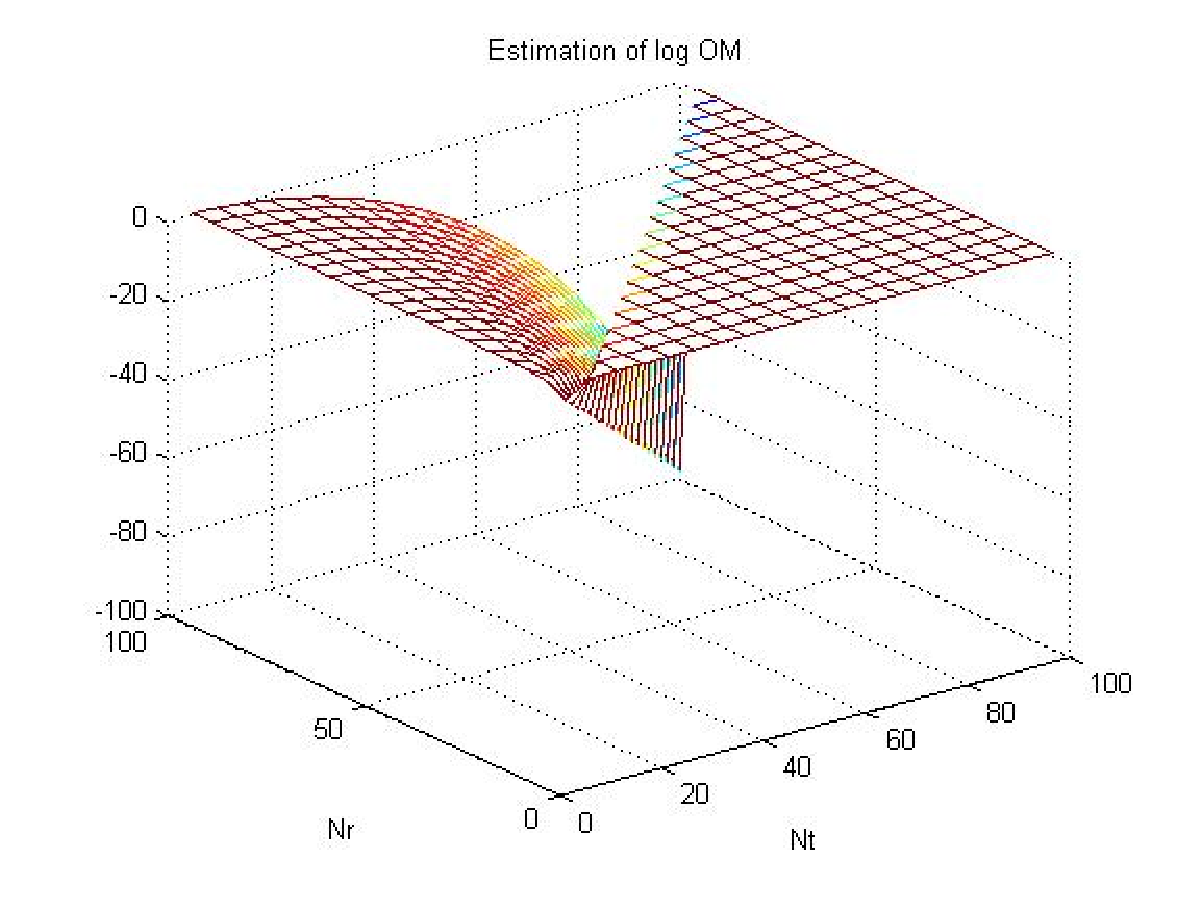
\includegraphics[width=0.7\textwidth, height=5cm]{logE_om_em.eps}
%\caption{Empirical Estimation $E[\ln(\phi_{om})]_{em}$}
%\label{figure1}
%\end{figure}

%\begin{figure}[htb]
%\centering
%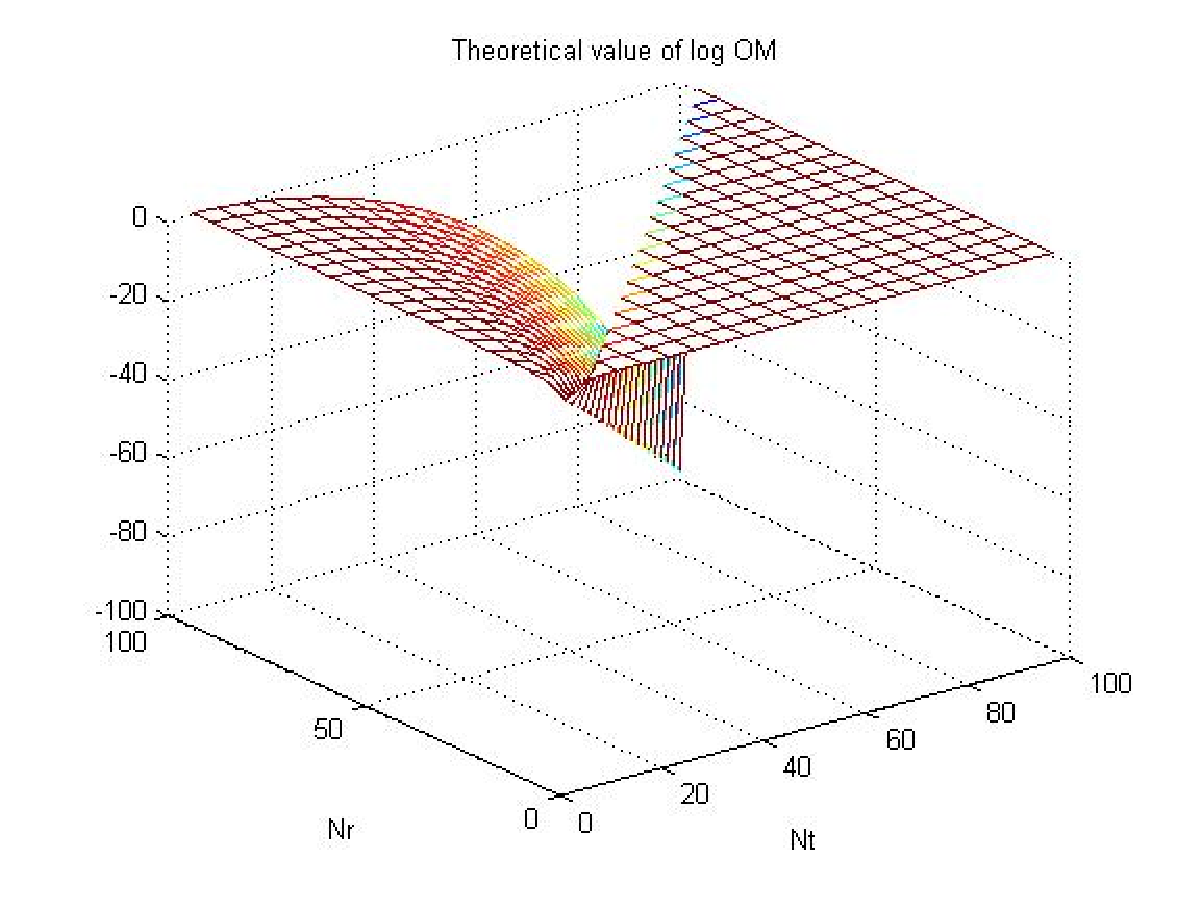
\includegraphics[width=0.7\textwidth, height=5cm]{logE_om_t.eps}
%\caption{Theoretical $E[\ln(\phi_{om})]_{t}$}
%\label{figure2}
%\end{figure} 


%\begin{figure}[htb]
%\centering
%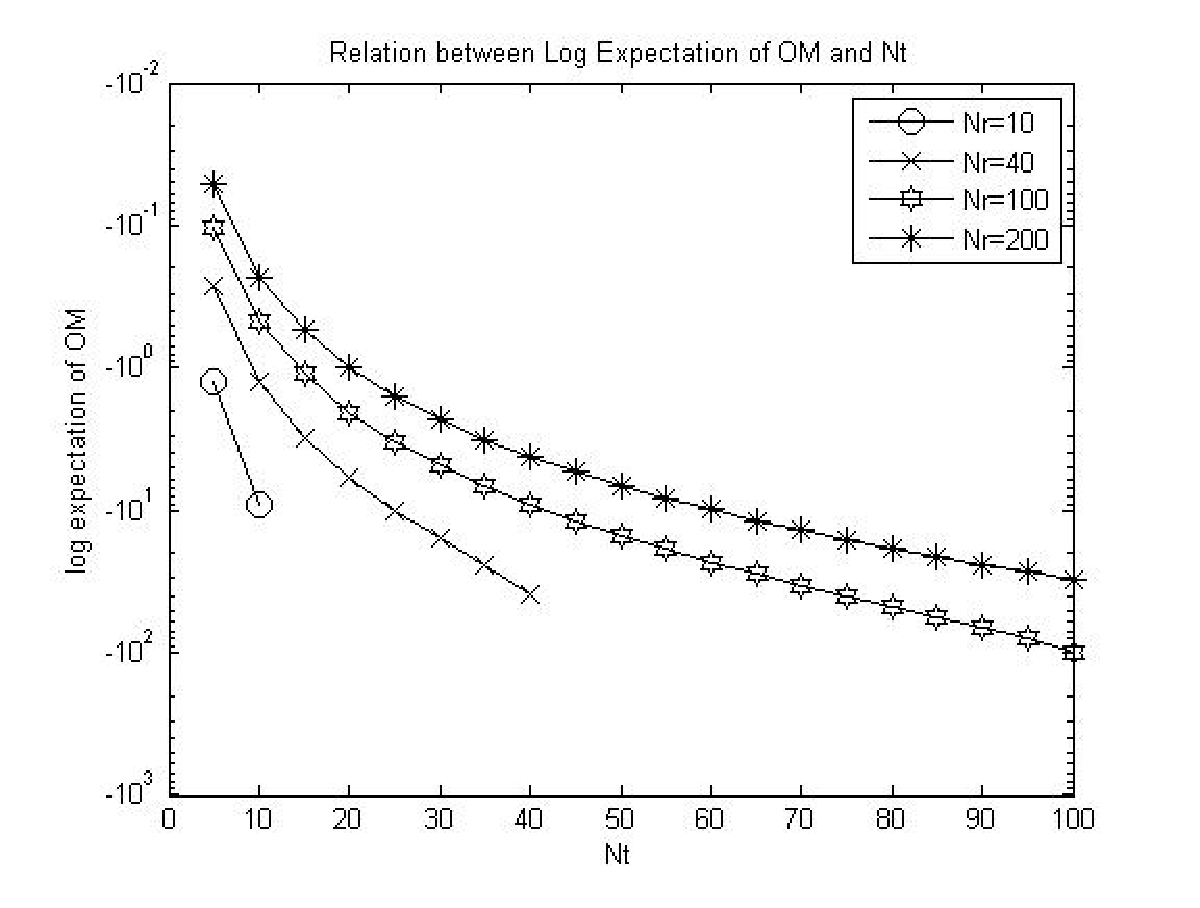
\includegraphics[scale=0.6]{NtE.eps}
%\caption{Relation between $N_{t}$ and $E[\ln(\phi_{om})]_{t}$}
%\label{figure3}
%\end{figure}

Fig.\ref{figure3} demonstrates the relation between the number of users ($N_{t}$) and $E[\ln(\phi_{om})]_{t}$ under cases of different numbers of antennas at base station ($N_{r}$). From Fig.\ref{figure3}, we can see, on the one hand, with $N_{r}$ fixed, $E[\ln(\phi_{om})]$ decreases while $N_{t}$ increases, however the gradient of each curve becomes more and more gentle. On the other hand, when $N_{r}$ becomes larger $E[\ln(\phi_{om})]$ becomes more insensitive to variation of $N_{t}$.
\section{Stopping Criteria}\label{stopping criteria}
As we have explained in section \ref{Introduce epsilon SVR}, the upper bound of Lagrangian dual objective function is determined by primal objective function further more the Lagrangian dual objective function equals to original objective function only when the optimal is found. Therefore, the gap between primal problem and dual problem is used to evaluate how is close is the current solution to global minimum. In our scenario, feasibility gap is employed as stopping criteria because of low computational cost and reliable performance.

  Based on the dual objective function in (\ref{final complex lagrange duality}) and the primal objective function in (\ref{complex objective function1}), based on the proposition of Lagrangian theorem
\begin{IEEEeqnarray}[\relax]{l}
\nonumber
 -\frac{1}{2}(\alpha-\hat{\alpha})^{T}\mathbf{K}^{r}(\alpha-\hat{\alpha})-\frac{1}{2}(\beta-\hat{\beta})^{T}\mathbf{K}^{r}(\beta-\hat{\beta})+Re(\mathbf{y}^{T})(\alpha-\hat{\alpha})+Im(\mathbf{y}^{T})(\beta-\hat{\beta})-\epsilon\mathbf{e}^{T}(\alpha+\hat{\alpha}+\beta+\hat{\beta})\\
+C\sum_{i=1}^{N_{r}}[\tilde{R}(\xi_{i}^{r})+\tilde{R}(\hat{\xi}_{i}^{r})+\tilde{R}(\xi_{i}^{i})+\tilde{R}(\hat{\xi}_{i}^{i})] \leq \frac{1}{2}||\mathbf{W}||^{2}_{\mathbb{H}}+C\sum_{i=1}^{N_{r}}[R(\xi_{i}^{r})+R(\hat{\xi}_{i}^{r})+R(\xi_{i}^{i})+R(\hat{\xi}_{i}^{i})]
\label{duality gap1}
\end{IEEEeqnarray}
 where $\mathbf{W}=\sum_{i=1}^{N_{r}}(\alpha_{i}-\hat{\alpha}_{i})\mathbf{h}_{i}-i\sum_{j=1}^{N_{r}}(\beta_{j}-\hat{\beta}_{j})\mathbf{h}_{j}$. The duality gap can be obtained by 
 \begin{IEEEeqnarray}[\relax]{l}
 \nonumber
 G(\alpha, \hat{\alpha}, \beta, \hat{\beta})=\frac{1}{2}||\mathbf{W}||^{2}_{\mathbb{H}}+C\sum_{i=1}^{N_{r}}[R(\xi_{i}^{r})+R(\hat{\xi}_{i}^{r})+R(\xi_{i}^{i})+R(\hat{\xi}_{i}^{i})]-\{-\frac{1}{2}(\alpha-\hat{\alpha})^{T}\mathbf{K}^{r}(\alpha-\hat{\alpha})\\
\nonumber 
 -\frac{1}{2}(\beta-\hat{\beta})^{T}\mathbf{K}^{r}(\beta-\hat{\beta})+Re(\mathbf{y}^{T})(\alpha-\hat{\alpha})+Im(\mathbf{y}^{T})(\beta-\hat{\beta})-\epsilon\mathbf{e}^{T}(\alpha+\hat{\alpha}+\beta+\hat{\beta})+C\sum_{i=1}^{N_{r}}[\tilde{R}(\xi_{i}^{r})+\tilde{R}(\hat{\xi}_{i}^{r})\\
 \nonumber
 +\tilde{R}(\xi_{i}^{i})+\tilde{R}(\hat{\xi}_{i}^{i})]\}=(\alpha-\hat{\alpha})^{T}\mathbf{K}^{r}(\alpha-\hat{\alpha}) +(\beta-\hat{\beta})^{T}\mathbf{K}^{r}(\beta-\hat{\beta})-Re(\mathbf{y}^{T})(\alpha-\hat{\alpha})-Im(\mathbf{y}^{T})(\beta-\hat{\beta})+\\
 \epsilon\mathbf{e}^{T}(\alpha+\hat{\alpha}+\beta+\hat{\beta})-(\alpha-\hat{\alpha})^{T}\mathbf{K}^{i}(\beta-\hat{\beta})+C\sum_{i=1}^{N_{r}}[\xi_{i}^{r}R^{'}(\xi_{i}^{r})+\hat{\xi}_{i}^{r}R^{'}(\hat{\xi}_{i}^{r})+\xi_{i}^{i}R^{'}(\xi_{i}^{i})+\hat{\xi}_{i}^{i}R^{'}(\hat{\xi}_{i}^{i})]
 \label{duality gap2}
 \end{IEEEeqnarray}
Because the noise is white Gaussian, therefore the optimal risk function is 
$R(\xi)=\frac{1}{2}\xi^{2}$, $\xi$ is the slack variable, hence 
\begin{equation}
\xi R^{'}(\xi)=\xi^{2},
\label{risk functional1}
\end{equation} 
\begin{equation}
\xi_{i}^{r}(\hat{\xi}^{r})=\max(0, |Re(y_{i})-Re(<\mathbf{h}_{i}, \mathbf{w}>_{\mathbb{H}})|-\epsilon),
\label{risk functional2}
\end{equation}
Because $\xi^{r}\hat{\xi}^{r}=0$ (estimation can only exceed $\epsilon$ tube in one direction), therefore there is only one of $\xi$ and $\hat{\xi}$ need to be considered, notice $Re(y_{i})-Re(<\mathbf{h}_{i}, \mathbf{W}>_{\mathbb{H}})=\Phi_{i}^{r}+\sum_{j=1}^{N_{r}}(\beta_{j}-\hat{\beta}_{j})\mathbf{K}^{i}_{ij}$ and $Im(y_{i})-Im(<\mathbf{h}_{i}, \mathbf{W}>_{\mathbb{H}})=\Phi_{i}^{i}-\sum_{j=1}^{N_{r}}(\alpha_{j}-\hat{\alpha}_{j})\mathbf{K}^{i}_{ij}$ hence the last term in (\ref{duality gap2}) can be rewritten as 
\begin{equation}
C\sum_{i=1}^{N_{r}}((|\Phi_{i}^{r}+\sum_{j=1}^{N_{r}}(\beta_{j}-\hat{\beta}_{j})\mathbf{K}^{i}_{ij}|)^{2}_{\epsilon}+(|\Phi_{i}^{i}-\sum_{j=1}^{N_{r}}(\alpha_{j}-\hat{\alpha}_{j})\mathbf{K}^{i}_{ij}|)^{2}_{\epsilon})
\label{risk functional3}
\end{equation}
where $()_{\epsilon}$ denotes $\epsilon$ insensitive function.
duality gap in (\ref{duality gap2}) can be divided into two part
\begin{equation}
G(\alpha, \hat{\alpha}, \beta, \hat{\beta})=L(\alpha, \hat{\alpha}, \beta, \hat{\beta})+S(\alpha, \hat{\alpha}, \beta, \hat{\beta}),
\label{divide duality gap}
\end{equation}
where 
\begin{equation}
L(\alpha, \hat{\alpha}, \beta, \hat{\beta})=(\alpha-\hat{\alpha})^{T}\mathbf{K}^{r}(\alpha-\hat{\alpha}) +(\beta-\hat{\beta})^{T}\mathbf{K}^{r}(\beta-\hat{\beta})-Re(\mathbf{y}^{T})(\alpha-\hat{\alpha})-Im(\mathbf{y}^{T})(\beta-\hat{\beta})+\epsilon\mathbf{e}^{T}(\alpha+\hat{\alpha}+\beta+\hat{\beta}),
\label{L sub function}
\end{equation}

\begin{equation}
S(\alpha, \hat{\alpha}, \beta, \hat{\beta})=C\sum_{i=1}^{N_{r}}((|\Phi_{i}^{r}+\sum_{j=1}^{N_{r}}(\beta_{j}-\hat{\beta}_{j})\mathbf{K}^{i}_{ij}|)^{2}_{\epsilon}+(|\Phi_{i}^{i}-\sum_{j=1}^{N_{r}}(\alpha_{j}-\hat{\alpha}_{j})\mathbf{K}^{i}_{ij}|)^{2}_{\epsilon})-(\alpha-\hat{\alpha})^{T}\mathbf{K}^{i}(\beta-\hat{\beta})
\label{S sub function}
\end{equation}
\section{Hyperparameter Setting}

\section{Computer Simulations}


% An example of a floating figure using the graphicx package.
% Note that \label must occur AFTER (or within) \caption.
% For figures, \caption should occur after the \includegraphics.
% Note that IEEEtran v1.7 and later has special internal code that
% is designed to preserve the operation of \label within \caption
% even when the captionsoff option is in effect. However, because
% of issues like this, it may be the safest practice to put all your
% \label just after \caption rather than within \caption{}.
%
% Reminder: the "draftcls" or "draftclsnofoot", not "draft", class
% option should be used if it is desired that the figures are to be
% displayed while in draft mode.
%
%\begin{figure}[!t]
%\centering
%\includegraphics[width=2.5in]{myfigure}
% where an .eps filename suffix will be assumed under latex, 
% and a .pdf suffix will be assumed for pdflatex; or what has been declared
% via \DeclareGraphicsExtensions.
%\caption{Simulation results for the network.}
%\label{fig_sim}
%\end{figure}

% Note that IEEE typically puts floats only at the top, even when this
% results in a large percentage of a column being occupied by floats.


% An example of a double column floating figure using two subfigures.
% (The subfig.sty package must be loaded for this to work.)
% The subfigure \label commands are set within each subfloat command,
% and the \label for the overall figure must come after \caption.
% \hfil is used as a separator to get equal spacing.
% Watch out that the combined width of all the subfigures on a 
% line do not exceed the text width or a line break will occur.
%
%\begin{figure*}[!t]
%\centering
%\subfloat[Case I]{\includegraphics[width=2.5in]{box}%
%\label{fig_first_case}}
%\hfil
%\subfloat[Case II]{\includegraphics[width=2.5in]{box}%
%\label{fig_second_case}}
%\caption{Simulation results for the network.}
%\label{fig_sim}
%\end{figure*}
%
% Note that often IEEE papers with subfigures do not employ subfigure
% captions (using the optional argument to \subfloat[]), but instead will
% reference/describe all of them (a), (b), etc., within the main caption.
% Be aware that for subfig.sty to generate the (a), (b), etc., subfigure
% labels, the optional argument to \subfloat must be present. If a
% subcaption is not desired, just leave its contents blank,
% e.g., \subfloat[].


% An example of a floating table. Note that, for IEEE style tables, the
% \caption command should come BEFORE the table and, given that table
% captions serve much like titles, are usually capitalized except for words
% such as a, an, and, as, at, but, by, for, in, nor, of, on, or, the, to
% and up, which are usually not capitalized unless they are the first or
% last word of the caption. Table text will default to \footnotesize as
% IEEE normally uses this smaller font for tables.
% The \label must come after \caption as always.
%
%\begin{table}[!t]
%% increase table row spacing, adjust to taste
%\renewcommand{\arraystretch}{1.3}
% if using array.sty, it might be a good idea to tweak the value of
% \extrarowheight as needed to properly center the text within the cells
%\caption{An Example of a Table}
%\label{table_example}
%\centering
%% Some packages, such as MDW tools, offer better commands for making tables
%% than the plain LaTeX2e tabular which is used here.
%\begin{tabular}{|c||c|}
%\hline
%One & Two\\
%\hline
%Three & Four\\
%\hline
%\end{tabular}
%\end{table}


% Note that the IEEE does not put floats in the very first column
% - or typically anywhere on the first page for that matter. Also,
% in-text middle ("here") positioning is typically not used, but it
% is allowed and encouraged for Computer Society conferences (but
% not Computer Society journals). Most IEEE journals/conferences use
% top floats exclusively. 
% Note that, LaTeX2e, unlike IEEE journals/conferences, places
% footnotes above bottom floats. This can be corrected via the
% \fnbelowfloat command of the stfloats package.




\section{Conclusion}
The conclusion goes here.





% if have a single appendix:
%\appendix[Proof of the Zonklar Equations]
% or
%\appendix  % for no appendix heading
% do not use \section anymore after \appendix, only \section*
% is possibly needed

% use appendices with more than one appendix
% then use \section to start each appendix
% you must declare a \section before using any
% \subsection or using \label (\appendices by itself
% starts a section numbered zero.)
%


\appendices
\section{Proof of the First Zonklar Equation}
Appendix one text goes here.

% you can choose not to have a title for an appendix
% if you want by leaving the argument blank
\section{}
Appendix two text goes here.
\section{}
Let $\mathbf{A}\in \mathbb{C}^{m\times m}$, $A\sim \mathbb{C}W(n, \mathbf{\Sigma})$, $\mathbb{C}W(n, \mathbf{\Sigma})$ denotes complex Wishart distribution with $n$ degrees of freedom and covariance matrix $\mathbf{\Sigma}$. It is obvious $\mathbf{A}$ is Hermition positive definite matrix, $\mathbf{A}=\mathbf{A}^{H}>0$.

The pdf of $\mathbf{A}$ can be written as\cite{nagar2011expectations}:
\begin{equation}
f(\mathbf{A})=\{\tilde{\Gamma}_{m}(n)det(\mathbf{\Sigma})^{n} \}^{-1}det(\mathbf{A})^{n-m}etr(-\mathbf{\Sigma}^{-1}\mathbf{A}),
\label{Appendequa1}
\end{equation}
where $\tilde{\Gamma}_{m}(\beta)$ denotes multivariate complex Gamma function defined by:
\begin{equation}
\tilde{\Gamma}_{m}(\beta)=\pi^{\frac{m(m-1)}{2}}\prod_{i=1}^{m}\Gamma(\beta-i+1)\quad Re(\beta)>m-1.
\label{Appendequa2}
\end{equation}
Furthermore, from \cite{nagar2011expectations}, we have 

\begin{equation}
\tilde{\Gamma}_{m}(\beta)=\int_{\mathbf{X}=\mathbf{X}^{H}>0}etr(-\mathbf{X})det(\mathbf{X})^{\beta-m}d
\mathbf{X} \quad Re(\beta)>m-1.
\label{Appendequa3}
\end{equation}
We derive logarithmic expectation of $det(\mathbf{A})$
\begin{eqnarray}
\nonumber
E[\ln(det(\mathbf{A}))]&=&\int_{\mathbf{A}=\mathbf{A}^{H}>0}\ln(det(\mathbf{A}))f(\mathbf{A})d\mathbf{A}\\
\nonumber
&=&\int_{\mathbf{A}=\mathbf{A}^{H}>0}\ln(det(\mathbf{A}))\{\tilde{\Gamma}_{m}(n)det(\mathbf{\Sigma})^{n} \}^{-1}det(\mathbf{A})^{n-m}etr(-\mathbf{\Sigma}^{-1}\mathbf{A})d\mathbf{A}\\
&=&\frac{det(\mathbf{\Sigma})^{-n}}{\tilde{\Gamma}_{m}(n)}\int_{\mathbf{A}=\mathbf{A}^{H}>0}\ln(det(\mathbf{A}))det(\mathbf{A})^{n-m}etr(-\mathbf{\Sigma}^{-1}\mathbf{A})d\mathbf{A},
\label{Appendequa4}
\end{eqnarray}
if $\mathbf{\Sigma}=\mathbf{I}$, (\ref{Appendequa4}) can be written as 
\begin{equation}
E[\ln(det(\mathbf{A}))]=\frac{1}{\tilde{\Gamma}_{m}(n)}\int_{\mathbf{A}=\mathbf{A}^{H}>0}\ln(det(\mathbf{A}))det(\mathbf{A})^{n-m}etr(-\mathbf{A})d\mathbf{A}.
\label{Appendequa5}
\end{equation}
Because $\frac{d}{dn}[det(\mathbf{A})]^{n-m}=\ln(det(\mathbf{A}))det(\mathbf{A})^{n-m}$, (\ref{Appendequa5}) can be rewritten as
\begin{equation}
E[\ln(det(\mathbf{A}))]=\frac{1}{\tilde{\Gamma}_{m}(n)}\frac{d}{dn}\int_{\mathbf{A}=\mathbf{A}^{H}>0}etr(-\mathbf{A})det(\mathbf{A})^{n-m}d\mathbf{A},
\label{Appendequa6}
\end{equation}
using (\ref{Appendequa3}), (\ref{Appendequa6}) can be rewritten as 
\begin{equation}
E[\ln(\mathbf{A})]=\frac{\tilde{\Gamma}^{'}_{m}(n)}{\tilde{\Gamma}_{m}(n)}.
\label{Appendequa7}
\end{equation}
Based on (\ref{Appendequa2}), we have 
\begin{equation}
\tilde{\Gamma}^{'}_{m}(n)=\pi^{\frac{m(m-1)}{2}}\sum_{i=1}^{m}[\Gamma^{'}(n-i+1)\prod_{j=1,j\neq i }^{m}\Gamma(n-j+1)],
\end{equation}
Thus we have 
\begin{equation}
E[\ln(det(\mathbf{A}))]=\frac{\tilde{\Gamma}^{'}_{m}(n)}{\tilde{\Gamma}_{m}(n)}=\sum_{i=1}^{m}\frac{\Gamma^{'}(n-i+1)}{\Gamma(n-i+1)}=\sum_{i=1}^{m}\psi(n-i+1),
\label{Appendequa8}
\end{equation}
where $\psi$ denotes Digamma function.
\section{}
If $x\sim Gamma(n, \theta)$, with shape parameter $k$ and scale parameter $\theta$, $x>0$, $\Gamma(k)$ denotes Gamma function, the density function of Gamma distribution is
\begin{equation}
f(x,k,\theta)=\frac{x^{k-1}e^{-x/\theta}}{\Gamma(k)\theta^{k}}.
\label{Appendequa9}
\end{equation}
Thus we have 
\begin{equation}
E[\ln(x)]=\frac{1}{\Gamma(k)}\int_{0}^{\infty}\ln(x)x^{k-1}e^{-x/\theta}\theta^{-k}dx,
\label{Appendequa10}
\end{equation}
define $z=x/\theta$ and since $\Gamma(k)=\int_{0}^{\infty}x^{k-1}e^{-x}dx$, (\ref{Appendequa10}) can be rewritten as
\begin{equation}
E[\ln(x)]=\ln(\theta)+\frac{1}{\Gamma(k)}\int_{0}^{\infty}\ln(z)z^{k-1}e^{-z}dz.
\label{Appendequa11}
\end{equation}
Because $\frac{d(z^{k-1})}{dk}=\ln(z)z^{k-1}$, (\ref{Appendequa11}) can be rewritten as
\begin{eqnarray}
\nonumber
E[\ln(z)]&=&\ln(\theta)+\frac{1}{\Gamma(k)}\frac{d}{dk}\int_{0}^{\infty}z^{k-1}e^{-z}dz\\
\nonumber
&=&\ln(\theta)+\frac{\Gamma^{'}(k)}{\Gamma(k)}\\
\nonumber
&=&\ln(\theta)+\psi(k),
\label{Appendequa12}
\end{eqnarray}
where $\psi(k)$ denotes Digamma function.
\section{}
$x_{1}, x_{2}, \cdots x_{N_{t}}$ are independent beta variables, the probability density function (pdf) can be written as: 
\begin{equation}
f(x_{i})=\frac{1}{\mathbb{B}(k_{1}^{i}, k_{2}^{i})}x_{i}^{k_{1}^{i}-1}(1-x_{i})^{k_{2}^{i}-1},
\label{Appendequal13}
\end{equation}
define $y_{i}=-\ln(x_{i})=g(x_{i})$, Based on Jacobian transformation, we have 
\begin{equation}
f_{y_{i}}(\rho)=|\frac{dy_{i}}{dx_{i}}|^{-1}f_{x_{i}}(g^{-1}(\rho))=\frac{1}{\mathbb{B}(k_{1}^{i},k_{2}^{i})}e^{-k_{1}^{i}\rho}(1-e^{-\rho})^{k_{2}^{i}-1}.
\label{Appendequal14}
\end{equation}
where (\ref{Appendequal14}) can be alternatively expressed as \cite{bhargava1981distribution}
\begin{equation}
f_{y_{i}}(\rho)=\sum_{j^{i}=0}^{k_{2}^{i}-1}c(k_{1}^{i},k_{2}^{i}, j^{i})(k_{1}^{i}+j^{i})exp(-(k_{1}^{i}+j^{i})\rho),
\label{Appendequal15}
\end{equation} 
where $c(k_{1}^{i}, k_{2}^{i}, j_{i})=(-1)^{j^{i}}$ $k_{2}^{i}-1\choose j^{i}$ $[(k_{1}^{i}+k_{2}^{i})\mathbb{B}(k_{1}^{i},k_{2}^{i})]^{-1}$, $\mathbb{B}(\alpha, \beta)$ denotes beta function. Based on the lemma 1 of \cite{bhargava1981distribution}, if $a_{1}, a_{2}, \cdots a_{n}$ are independent exponentially distributed random variables, with pdf given by
\begin{equation}
t_{i}exp(-t_{i}a_{i}),
\label{Appendequal16}
\end{equation} 
then pdf of $a=\sum_{i=1}^{n}a_{i}$ can be written as
\begin{equation}
f(a|\mathbf{t})=\prod_{i=1}^{n}t_{i}\sum_{i=1}^{n}[exp(-t_{i}a)/\prod_{j=1\\ j\neq i}^{j=n}(t_{j}-t_{i})],
\label{Appendequal17}
\end{equation}
where $t=[t_{1}, t_{2}, \cdots t_{n}]$. The pdf of $y_{i}$ can be viewed as the weighting summation of exponential distribution functions, define $y=\sum_{i=1}^{n}y_{i}$, based on (\ref{Appendequal17}), the pdf of $y$ is given by
\begin{equation}
f_{y}(m)=\sum_{\mathbf{j}}\{[\prod_{i=1}^{n}c(k_{1}^{i},k_{2}^{i}, j^{i})]f(m|\mathbf{k_{1}}+\mathbf{j})\},
\label{Appendequal18}
\end{equation}
where $\sum_{\mathbf{j}}=\sum_{j^{1}}\sum_{j^{2}}\cdots \sum_{j^{n}}$, the range of $j^{i}$ is defined by $j^{i}\in [0, k_{2}^{i}]$, $f(m|\mathbf{k_{1}}+\mathbf{j})=(\prod_{i=1}^{N_{t}}(k_{1}^{i}+j^{i}))\sum_{i=1}^{N_{t}}[exp(-(k_{1}^{i}+j^{i})m)/\prod_{j=1\\ j\neq i}^{N_{t}}(k_{1}^{j}+j^{j}-k_{1}^{i}-j^{i})]$, $\mathbf{k_{1}}+\mathbf{j}=[k_{1}^{1}+j^{1}, k_{1}^{2}+j^{2} \cdots k_{1}^{n}+j^{n}]$. we define $U=exp(-y)=\prod_{i=1}^{n}x_{i}$, using Jacobian transformation, the pdf of $U$ is given by 
\begin{equation}
f_{U}(u)=|\frac{du}{dy}|^{-1}f_{y}(-\ln(u))=\frac{1}{u}\sum_{\mathbf{j}}\{[\prod_{i=1}^{n}c(k_{1}^{i},k_{2}^{i},j^{i})]f(-\ln(u)|\mathbf{k_{1}}+\mathbf{j})\}.
\label{Appendequal19}
\end{equation}

% use section* for acknowledgment
%\section*{Acknowledgment}


%The authors would like to thank...


% Can use something like this to put references on a page
% by themselves when using endfloat and the captionsoff option.
\ifCLASSOPTIONcaptionsoff
  \newpage
\fi



% trigger a \newpage just before the given reference
% number - used to balance the columns on the last page
% adjust value as needed - may need to be readjusted if
% the document is modified later
%\IEEEtriggeratref{8}
% The "triggered" command can be changed if desired:
%\IEEEtriggercmd{\enlargethispage{-5in}}

% references section

% can use a bibliography generated by BibTeX as a .bbl file
% BibTeX documentation can be easily obtained at:
% http://www.ctan.org/tex-archive/biblio/bibtex/contrib/doc/
% The IEEEtran BibTeX style support page is at:
% http://www.michaelshell.org/tex/ieeetran/bibtex/
%\bibliographystyle{IEEEtran}
% argument is your BibTeX string definitions and bibliography database(s)
%\bibliography{IEEEabrv,../bib/paper}
%
% <OR> manually copy in the resultant .bbl file
% set second argument of \begin to the number of references
% (used to reserve space for the reference number labels box)
%\begin{thebibliography}{1}

%\bibitem{IEEEhowto:kopka}
%H.~Kopka and P.~W. Daly, \emph{A Guide to \LaTeX}, 3rd~ed.\hskip 1em plus
%  0.5em minus 0.4em\relax Harlow, England: Addison-Wesley, 1999.

%\end{thebibliography}

% biography section
% 
% If you have an EPS/PDF photo (graphicx package needed) extra braces are
% needed around the contents of the optional argument to biography to prevent
% the LaTeX parser from getting confused when it sees the complicated
% \includegraphics command within an optional argument. (You could create
% your own custom macro containing the \includegraphics command to make things
% simpler here.)
%\begin{IEEEbiography}[{\includegraphics[width=1in,height=1.25in,clip,keepaspectratio]{mshell}}]{Michael Shell}
% or if you just want to reserve a space for a photo:

%\begin{IEEEbiography}{Michael Shell}
%Biography text here.
%\end{IEEEbiography}

% if you will not have a photo at all:
%\begin{IEEEbiographynophoto}{John Doe}
%Biography text here.
%\end{IEEEbiographynophoto}

% insert where needed to balance the two columns on the last page with
% biographies
%\newpage

%\begin{IEEEbiographynophoto}{Jane Doe}
%Biography text here.
%\end{IEEEbiographynophoto}

% You can push biographies down or up by placing
% a \vfill before or after them. The appropriate
% use of \vfill depends on what kind of text is
% on the last page and whether or not the columns
% are being equalized.

%\vfill

% Can be used to pull up biographies so that the bottom of the last one
% is flush with the other column.
%\enlargethispage{-5in}



% that's all folks
%\end{spacing}
\newpage
\bibliographystyle{IEEEtran}
\bibliography{citation}
\end{document}


